\documentclass[11pt,preprint]{elsarticle}

\usepackage{lmodern}
%%%% My spacing
\usepackage{setspace}
\setstretch{1.2}
\DeclareMathSizes{12}{14}{10}{10}

% Wrap around which gives all figures included the [H] command, or places it "here". This can be tedious to code in Rmarkdown.
\usepackage{float}
% The [H] wrapper for figures is switched off, so that figures float to the top or bottom of a page as set by fig.pos in the Rmd and pages are not left half empty
% \let\origfigure\figure
% \let\endorigfigure\endfigure
% \renewenvironment{figure}[1][2] {
%     \expandafter\origfigure\expandafter[H]
% } {
%     \endorigfigure
% }

\let\origtable\table
\let\endorigtable\endtable
\renewenvironment{table}[1][2] {
    \expandafter\origtable\expandafter[H]
} {
    \endorigtable
}


\usepackage{ifxetex,ifluatex}
\usepackage{fixltx2e} % provides \textsubscript
\ifnum 0\ifxetex 1\fi\ifluatex 1\fi=0 % if pdftex
  \usepackage[T1]{fontenc}
  \usepackage[utf8]{inputenc}
\else % if luatex or xelatex
  \ifxetex
    \usepackage{mathspec}
    \usepackage{xltxtra,xunicode}
  \else
    \usepackage{fontspec}
  \fi
  \defaultfontfeatures{Mapping=tex-text,Scale=MatchLowercase}
  \newcommand{\euro}{€}
\fi

\usepackage{amssymb, amsmath, amsthm, amsfonts}

\def\bibsection{\section*{References}} %%% Make "References" appear before bibliography


\usepackage[numbers]{natbib}

\usepackage{longtable}
\usepackage[margin=2.3cm,bottom=2cm,top=2.5cm, includefoot]{geometry}
\usepackage{fancyhdr}
\usepackage[bottom, hang, flushmargin]{footmisc}
\usepackage{graphicx}
\numberwithin{equation}{section}
\numberwithin{figure}{section}
\numberwithin{table}{section}
\setlength{\parindent}{0cm}
\setlength{\parskip}{1.3ex plus 0.5ex minus 0.3ex}
\usepackage{textcomp}
\renewcommand{\headrulewidth}{0.2pt}
\renewcommand{\footrulewidth}{0.3pt}

\usepackage{array}
\newcolumntype{x}[1]{>{\centering\arraybackslash\hspace{0pt}}p{#1}}

%%%%  Remove the "preprint submitted to" part. Don't worry about this either, it just looks better without it:
\makeatletter
\def\ps@pprintTitle{%
  \let\@oddhead\@empty
  \let\@evenhead\@empty
  \let\@oddfoot\@empty
  \let\@evenfoot\@oddfoot
}
\makeatother

 \def\tightlist{} % This allows for subbullets!

\usepackage{hyperref}
\hypersetup{breaklinks=true,
            bookmarks=true,
            colorlinks=true,
            citecolor=blue,
            urlcolor=blue,
            linkcolor=blue,
            pdfborder={0 0 0}}


% The following packages allow huxtable to work:
\usepackage{siunitx}
\usepackage{multirow}
\usepackage{hhline}
\usepackage{calc}
\usepackage{tabularx}
\usepackage{booktabs}
\usepackage{caption}


\newenvironment{columns}[1][]{}{}

\newenvironment{column}[1]{\begin{minipage}{#1}\ignorespaces}{%
\end{minipage}
\ifhmode\unskip\fi
\aftergroup\useignorespacesandallpars}

\def\useignorespacesandallpars#1\ignorespaces\fi{%
#1\fi\ignorespacesandallpars}

\makeatletter
\def\ignorespacesandallpars{%
  \@ifnextchar\par
    {\expandafter\ignorespacesandallpars\@gobble}%
    {}%
}
\makeatother


% definitions for citeproc citations
\NewDocumentCommand\citeproctext{}{}
\NewDocumentCommand\citeproc{mm}{%
\href{\#cite.\detokenize{#1}}{#2}\nocite{#1}}

\makeatletter
% allow citations to break across lines
\let\@cite@ofmt\@firstofone
% avoid brackets around text for \cite:
\def\@biblabel#1{}
\def\@cite#1#2{{#1\if@tempswa , #2\fi}}
\makeatother
\newlength{\cslhangindent}
\setlength{\cslhangindent}{1.5em}
\newlength{\csllabelwidth}
\setlength{\csllabelwidth}{3em}
\newenvironment{CSLReferences}[2] % #1 hanging-indent, #2 entry-spacing
{\begin{list}{}{%
	\setlength{\itemindent}{0pt}
	\setlength{\leftmargin}{0pt}
	\setlength{\parsep}{0pt}
	% turn on hanging indent if param 1 is 1
	\ifodd #1
	\setlength{\leftmargin}{\cslhangindent}
	\setlength{\itemindent}{-1\cslhangindent}
	\fi
	% set entry spacing
	\setlength{\itemsep}{#2\baselineskip}}}
{\end{list}}

\usepackage{calc}
\newcommand{\CSLBlock}[1]{\hfill\break\parbox[t]{\linewidth}{\strut\ignorespaces#1\strut}}
\newcommand{\CSLLeftMargin}[1]{\parbox[t]{\csllabelwidth}{\strut#1\strut}}
\newcommand{\CSLRightInline}[1]{\parbox[t]{\linewidth - \csllabelwidth}{\strut#1\strut}}
\newcommand{\CSLIndent}[1]{\hspace{\cslhangindent}#1}


\urlstyle{same}  % don't use monospace font for urls
\setlength{\parindent}{0pt}
\setlength{\parskip}{6pt plus 2pt minus 1pt}
\setlength{\emergencystretch}{3em}  % prevent overfull lines
\setcounter{secnumdepth}{5}

%%% Use protect on footnotes to avoid problems with footnotes in titles
\let\rmarkdownfootnote\footnote%
\def\footnote{\protect\rmarkdownfootnote}
\IfFileExists{upquote.sty}{\usepackage{upquote}}{}

%%% Include extra packages specified by user
\renewcommand{\topfraction}{0.9}
\renewcommand{\bottomfraction}{0.8}
\renewcommand{\textfraction}{0.07}
\renewcommand{\floatpagefraction}{0.8}
\setcounter{topnumber}{2}
\setcounter{bottomnumber}{2}
\setcounter{totalnumber}{3}
\usepackage{placeins}

%%% Hard setting column skips for reports - this ensures greater consistency and control over the length settings in the document.
%% page layout
%% paragraphs
\setlength{\baselineskip}{12pt plus 0pt minus 0pt}
\setlength{\parskip}{12pt plus 0pt minus 0pt}
\setlength{\parindent}{0pt plus 0pt minus 0pt}
%% floats
\setlength{\floatsep}{12pt plus 0 pt minus 0pt}
\setlength{\textfloatsep}{20pt plus 0pt minus 0pt}
\setlength{\intextsep}{14pt plus 0pt minus 0pt}
\setlength{\dbltextfloatsep}{20pt plus 0pt minus 0pt}
\setlength{\dblfloatsep}{14pt plus 0pt minus 0pt}
%% maths
\setlength{\abovedisplayskip}{12pt plus 0pt minus 0pt}
\setlength{\belowdisplayskip}{12pt plus 0pt minus 0pt}
%% lists
\setlength{\topsep}{10pt plus 0pt minus 0pt}
\setlength{\partopsep}{3pt plus 0pt minus 0pt}
\setlength{\itemsep}{5pt plus 0pt minus 0pt}
\setlength{\labelsep}{8mm plus 0mm minus 0mm}
\setlength{\parsep}{\the\parskip}
\setlength{\listparindent}{\the\parindent}
%% verbatim
\setlength{\fboxsep}{5pt plus 0pt minus 0pt}



\begin{document}



\begin{frontmatter}  %

\title{Exploring Risk and Uncertainty in the Local Equity Market}

% Set to FALSE if wanting to remove title (for submission)




\author[Add1]{Diaz Sangeve}
\ead{24991422@sun.ac.za}





\address[Add1]{Stellenbosch University, Stellenbosch, South Africa}

\cortext[cor]{Corresponding author: Diaz Sangeve}

\begin{abstract}
\small{
This paper examines how offshore economic and policy uncertainty has
affected volatility on the Johannesburg Stock Exchange and what it
implies for building risk ballasts into local equity funds. Local
volatility rose sharply in 2026, but as a temporary episode that
mirrored emerging markets and the oil market, while developed market
volatility stayed below its average. The firm's SafeCore fund
outperformed its Capped SWIX benchmark by 2.5 percentage points a year,
yet it ran slightly more volatility than the benchmark on most days,
offered no protection in stressed regimes and carried no low volatility
exposure, with two gold miners generating 45 percent of its risk by
August 2026. Own momentum and low volatility scores identify the local
strategy indexes correctly, while the vendor's volatility score does
not. Alpha opportunity since 2020 has been episodic, and the oil and
bond market volatility that transmits offshore shocks also raises
correlations among the largest local stocks, compressing the room for
active management.
}
\end{abstract}

\vspace{1cm}


\begin{keyword}
\footnotesize{
Volatility \sep GARCH \sep Dispersion \sep Factor scores \sep Active
management \\
\vspace{0.3cm}
}
\footnotesize{
\textit{JEL classification} G11 \sep G12 \sep C58
}
\end{keyword}



\vspace{0.5cm}

\end{frontmatter}

\setcounter{footnote}{0}



%________________________
% Header and Footers
%%%%%%%%%%%%%%%%%%%%%%%%%%%%%%%%%
\pagestyle{fancy}
\chead{}
\rhead{}
\lfoot{}
\rfoot{\footnotesize Page \thepage}
\lhead{}
%\rfoot{\footnotesize Page \thepage } % "e.g. Page 2"
\cfoot{}

%\setlength\headheight{30pt}
%%%%%%%%%%%%%%%%%%%%%%%%%%%%%%%%%
%________________________

\headsep 35pt % So that header does not go over title




\section{\texorpdfstring{Introduction
\label{Intro}}{Introduction }}\label{introduction}

A recent seminar argued that oil price volatility and global policy
uncertainty are feeding into local equity markets, and that local funds
should hold more low volatility stocks as a ballast. This paper tests
that argument in three steps. Section \ref{PartA} establishes whether
volatility on the local exchange has increased and whether the increase
mirrors the global experience. Section \ref{PartB} evaluates whether the
firm's SafeCore fund, which is built without reference to volatility,
has managed volatility well, where its risk comes from and what factor
exposures it holds. Section \ref{PartC} measures the alpha opportunity
in the local market since 2020 and relates it to global macro variables.
Section \ref{Conclusion} draws the implications together.

\section{\texorpdfstring{Data and Methods
\label{Data}}{Data and Methods }}\label{data-and-methods}

The analysis uses daily returns for the Capped SWIX, the Top 40, mid cap
and small cap indexes from 2015, the MSCI All Country World and Emerging
Markets indexes in dollars, daily stock returns, monthly holdings for
SafeCore and the Capped SWIX, daily Capped SWIX constituents from August
2020, a set of global volatility and uncertainty gauges, and monthly
returns for South African active managers. The Capped SWIX serves as the
local yardstick throughout, since it is SafeCore's benchmark. Daily
stock returns are capped at 25 percent when building portfolios and at
50 percent when measuring dispersion, since the data contains a handful
of implausible values. The methods include rolling realised volatility,
GARCH and DCC models, stratification by global regime, portfolio returns
from holdings, marginal risk contributions and cross-sectional
dispersion.

\section{\texorpdfstring{Local Volatility in a Global Context
\label{PartA}}{Local Volatility in a Global Context }}\label{local-volatility-in-a-global-context}

\subsection{Scope and Method}\label{scope-and-method}

This part establishes whether volatility on the local exchange has
increased and whether that increase mirrors the global experience. The
analysis moves from simple measures to model-based ones. It first
compares annualised volatility across sub-periods and traces its timing
with rolling windows and a monthly heatmap. It then separates the
volatility signal from noise using GARCH models, examines how strongly
volatility responds to bad news, and uses a DCC model to test whether
the local market has become more tightly linked to global markets.
Finally, it stratifies the sample by global conditions to identify which
external forces local volatility responds to, and which local segment
holds up best when they strike.

Three choices shape the analysis. The Capped SWIX (J433) serves as the
local yardstick, since it is the fund's benchmark in Part B and its
capping prevents a handful of large shares from dominating the result.
The MSCI All Country World index represents the global experience, while
the MSCI Emerging Markets index represents the peer group to which South
Africa belongs. The local index is quoted in rand and the MSCI indexes
in dollars, and each is kept in its own currency because the question
concerns the volatility that each investor base experiences. Part of any
difference between them may therefore reflect movements in the rand.

\subsection{Volatility by Period}\label{volatility-by-period}

The most direct test compares annualised volatility across periods. The
sample is divided into the calm years before Covid, the Covid year
itself, the recovery from 2021 to 2024, and 2025 and 2026 separately,
since these two years are the focus of the seminar. The shift chart
below tracks how each index moved from its 2021 to 2024 baseline into
2026, with the grey diamond marking its full sample norm and the change
in percentage points displayed in the right-hand column.

\begin{figure}[H]

{\centering 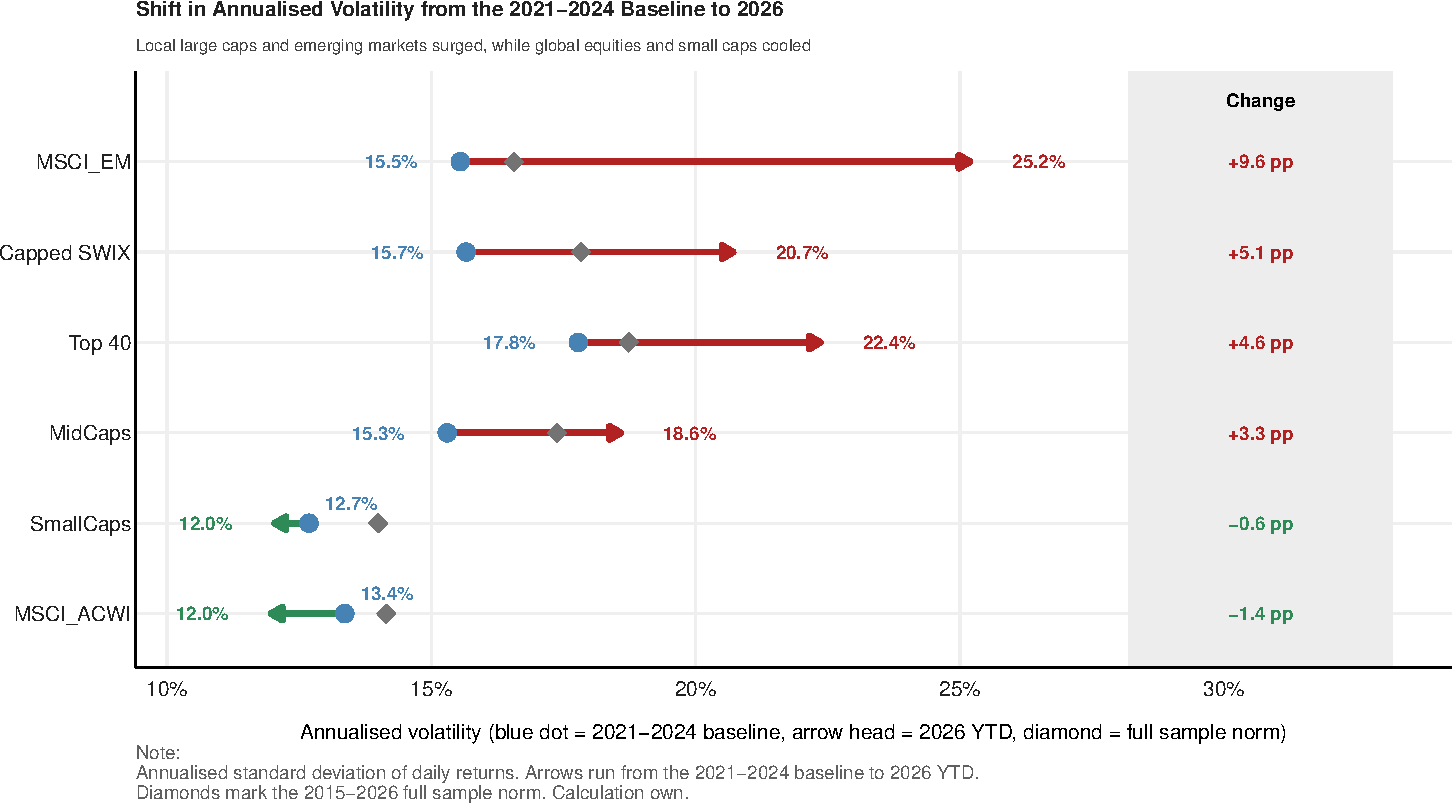
\includegraphics[width=1\linewidth]{Question1_files/figure-latex/q1a_period_shift-1} 

}

\caption{Shift in Annualised Volatility from the 2021-2024 Baseline to 2026}\label{fig:q1a_period_shift}
\end{figure}

The figure shows that local volatility rose in 2026 while global
volatility did not. The Capped SWIX recorded annualised volatility of
20.7 percent in 2026, above the 15.7 percent of 2021 to 2024 and its
full sample level of 17.8 percent. The MSCI ACWI moved in the opposite
direction, at 12.0 percent in 2026 against a full sample level of 14.1
percent, while the MSCI Emerging Markets index rose to 25.2 percent. The
rise in local volatility therefore resembles the emerging market
experience far more closely than the global one. Small caps are an
exception, with volatility of 12.0 percent in 2026 against 14.0 percent
over the full sample, which suggests that the turbulence was
concentrated in the larger and more globally exposed shares of the Top
40, where volatility reached 22.4 percent.

\subsection{Rolling Realised
Volatility}\label{rolling-realised-volatility}

\begin{figure}[H]

{\centering 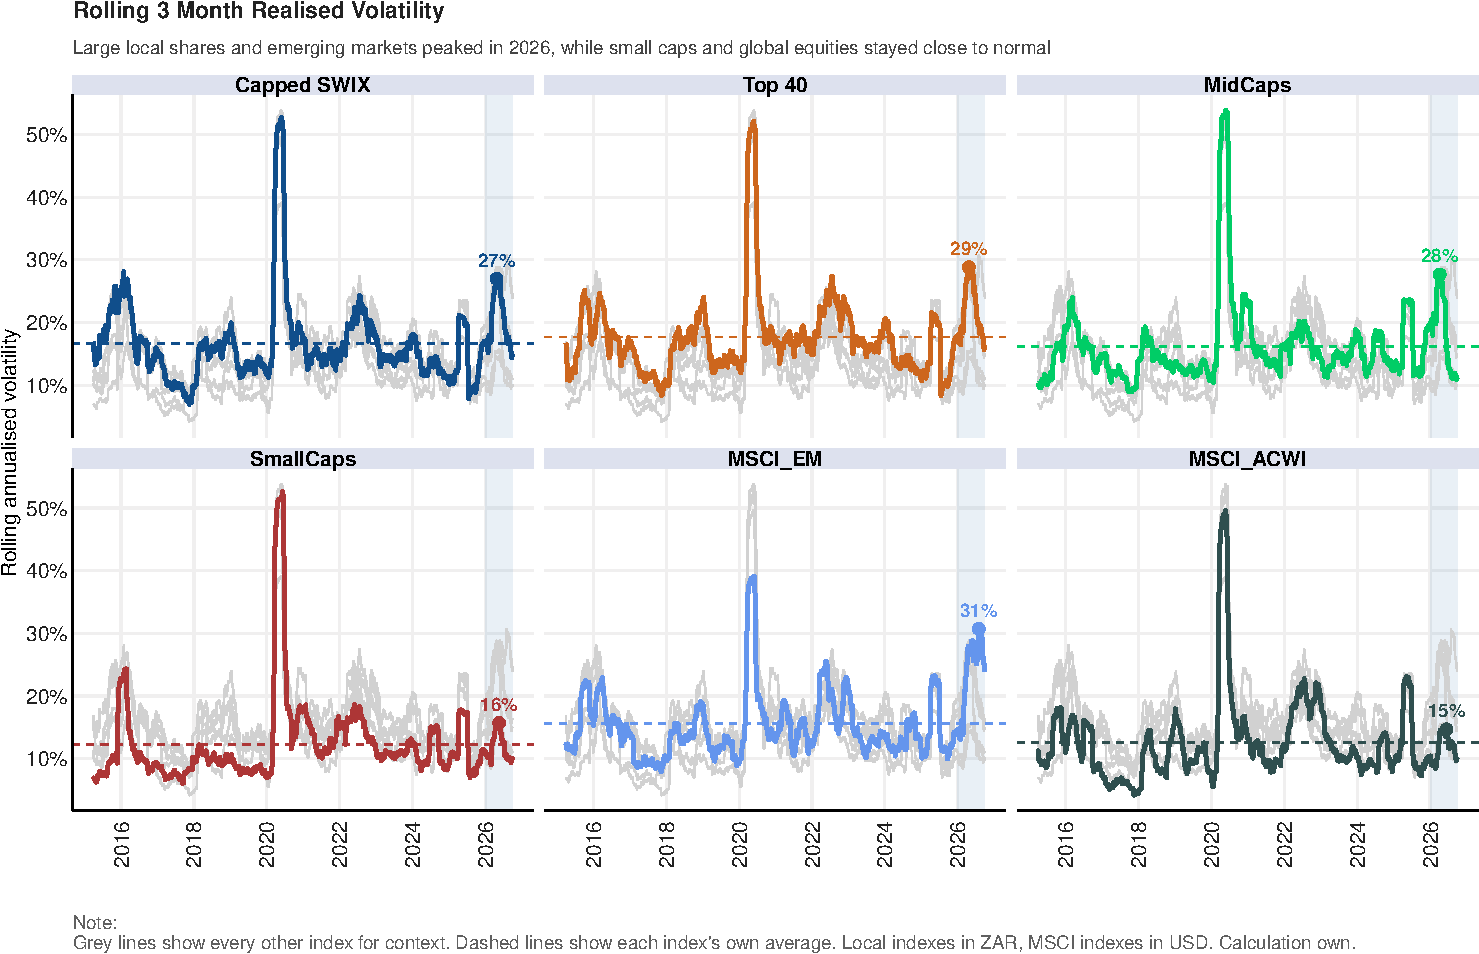
\includegraphics[width=1\linewidth]{Question1_files/figure-latex/q1a_rolling-1} 

}

\caption{Rolling 3 Month Realised Volatility}\label{fig:q1a_rolling}
\end{figure}

Figure \ref{fig:q1a_rolling} traces three month rolling volatility.
Local volatility peaked in April 2026 and had fallen back to 15 percent
by September, while small caps and the global index barely moved. The
2026 rise was therefore a pronounced but temporary episode.

\subsection{A Heatmap of Monthly
Volatility}\label{a-heatmap-of-monthly-volatility}

\begin{figure}[H]

{\centering 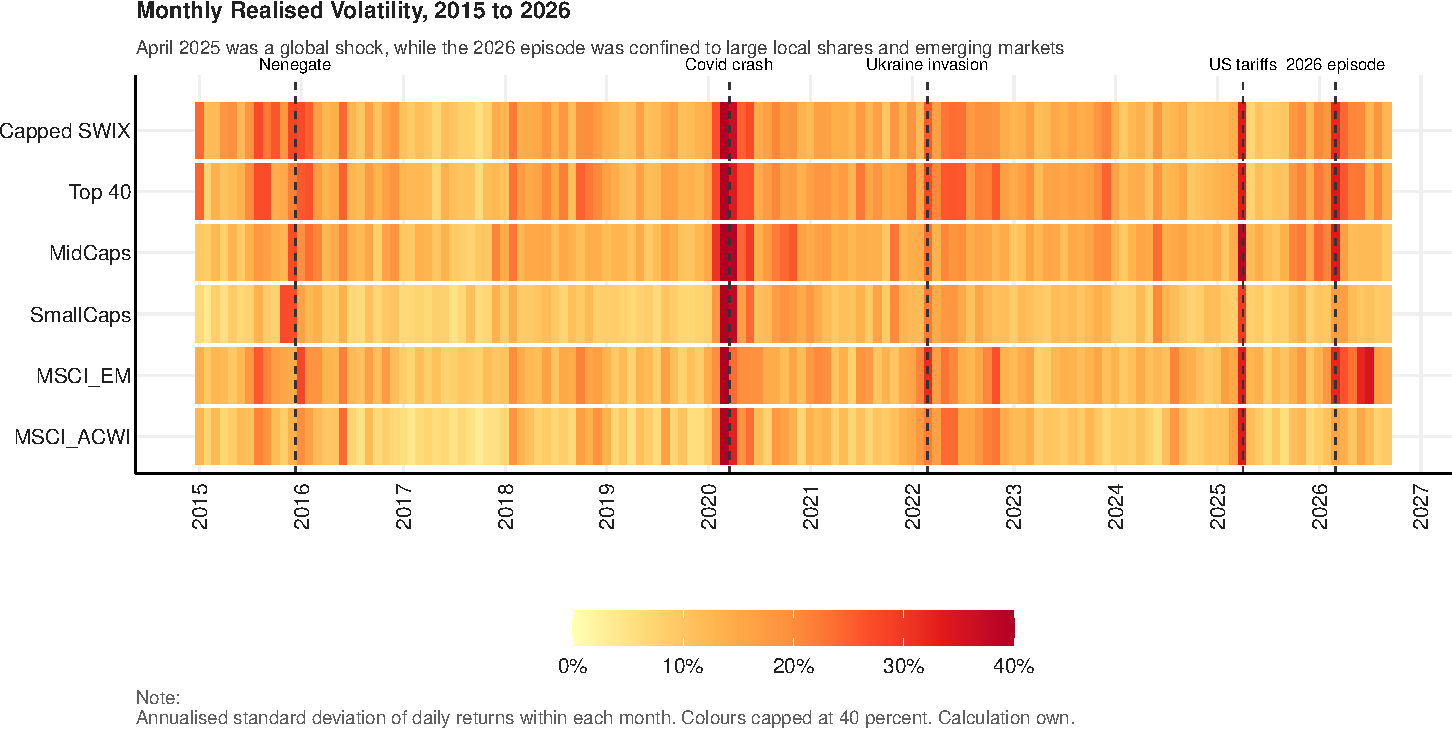
\includegraphics[width=1\linewidth]{Question1_files/figure-latex/q1a_heatmap-1} 

}

\caption{Monthly Realised Volatility, 2015 to 2026}\label{fig:q1a_heatmap}
\end{figure}

Figure \ref{fig:q1a_heatmap} shows the reach of each episode. The US
tariff announcements of April 2025 darken every row, which marks them as
a global shock. March 2026 was the 4th most volatile month on the Capped
SWIX since 2015, at 31.9 percent, but the global and small cap rows stay
pale through 2026.

\subsection{Volatility Clustering in Daily
Returns}\label{volatility-clustering-in-daily-returns}

Before a GARCH model is fitted, the data should show the feature it is
built to capture. The autocorrelation of daily returns is compared with
the autocorrelation of squared returns for the local, global and
emerging market indexes, with the Ljung-Box test over ten lags reported
in each panel.

\begin{figure}[H]

{\centering 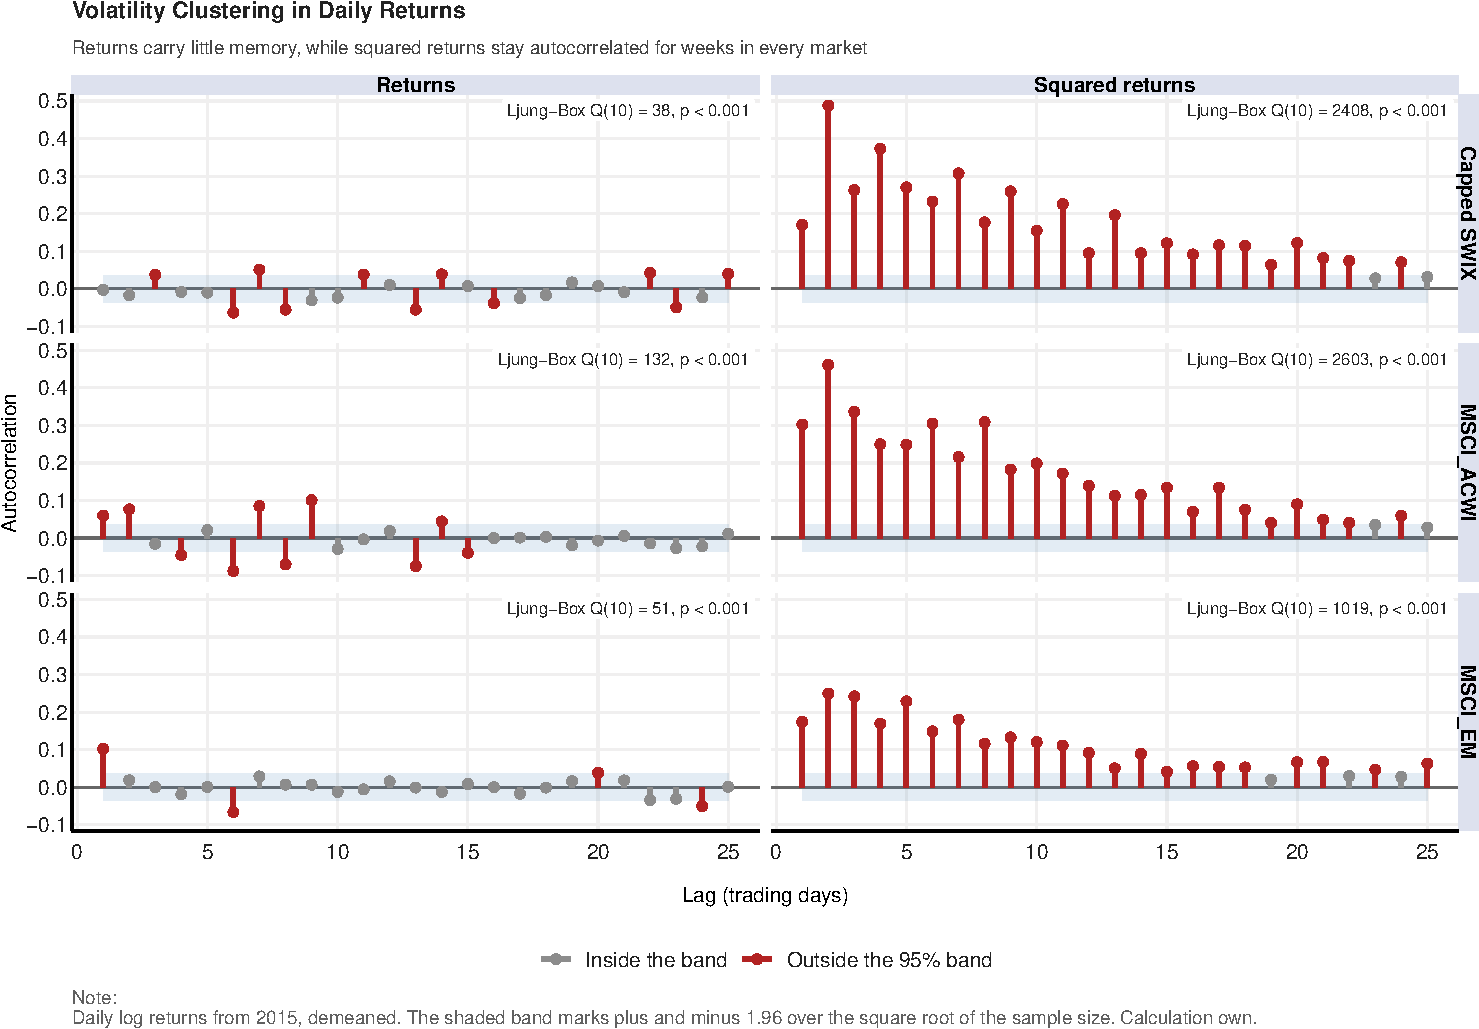
\includegraphics[width=1\linewidth]{Question1_files/figure-latex/q1a_acf-1} 

}

\caption{Volatility Clustering in Daily Returns}\label{fig:q1a_acf}
\end{figure}

Returns themselves carry little memory. Between 4 and 11 of the 25 lags
fall outside the band, and every one of those autocorrelations is small.
The Ljung-Box test still rejects the absence of autocorrelation for all
three series, with a statistic of 38 locally and 132 globally. The
global figure is the largest because the MSCI ACWI combines markets that
close at different times, so news that reaches Asia after New York has
closed enters the index a day late. Squared returns behave very
differently. Their autocorrelation is positive at almost every lag, with
22 to 23 of the 25 lags outside the band, and the Ljung-Box statistic
rises to 2408 for the Capped SWIX. Large moves tend to follow large
moves in every market, which is the clustering a GARCH model is designed
to capture, and the small autocorrelation in returns themselves supports
the AR(1) mean equation used below.

\subsection{Conditional Volatility from GARCH
Models}\label{conditional-volatility-from-garch-models}

Realised volatility has a mechanical weakness, since a single large
return remains in the window for three months and then drops out
abruptly. A GARCH model avoids this by separating the volatility signal
from the noise in returns. To avoid imposing a specification, the
function fits four candidate models to each index, namely the standard
GARCH, GJR, EGARCH and APARCH, each with an AR(1) mean equation and
student t errors, and retains the model with the lowest AIC. The
ridgeline plot then shows the full distribution of each index's daily
conditional volatility within every year, with a line at each year's
median, which shows shifts in the whole distribution that a single
average would hide.

\begin{figure}[H]

{\centering 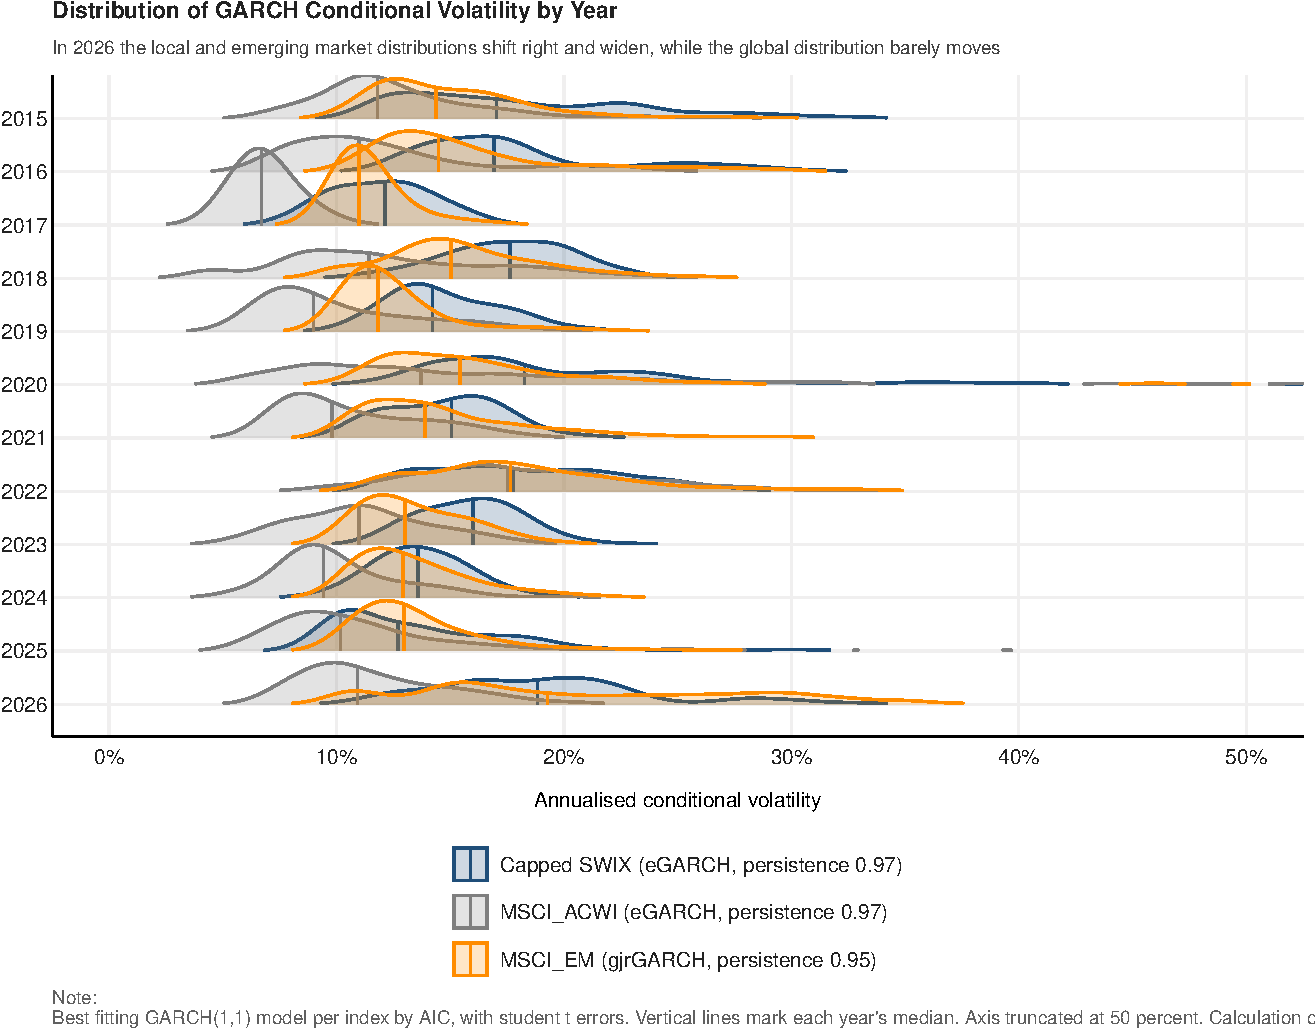
\includegraphics[width=1\linewidth]{Question1_files/figure-latex/q1a_garch-1} 

}

\caption{Distribution of GARCH Conditional Volatility by Year}\label{fig:q1a_garch}
\end{figure}

The data favour asymmetric models for all three indexes, as the legend
shows, with an EGARCH selected for the Capped SWIX and the global index
and a GJR model for emerging markets. Asymmetry means that negative
shocks raise volatility by more than positive shocks of the same size,
so volatility tends to arrive when returns are already falling.
Persistence of 0.97 for the Capped SWIX implies that half of a
volatility shock is still present after roughly 24 trading days. Through
most of the sample the global distribution sits to the left of the other
two, reflecting its lower base level of volatility. In 2026 the local
and emerging market distributions shift to the right and spread out,
while the global distribution stays close to its usual position. Local
conditional volatility averaged 19.1 percent in 2026 against 16.5
percent over the full sample, while global conditional volatility
averaged 11.6 percent, slightly below its own norm of 12.2 percent. With
the noise removed, the GARCH estimates confirm the pattern found in
realised volatility.

\subsection{The Asymmetric Response to Bad
News}\label{the-asymmetric-response-to-bad-news}

\begin{figure}[H]

{\centering 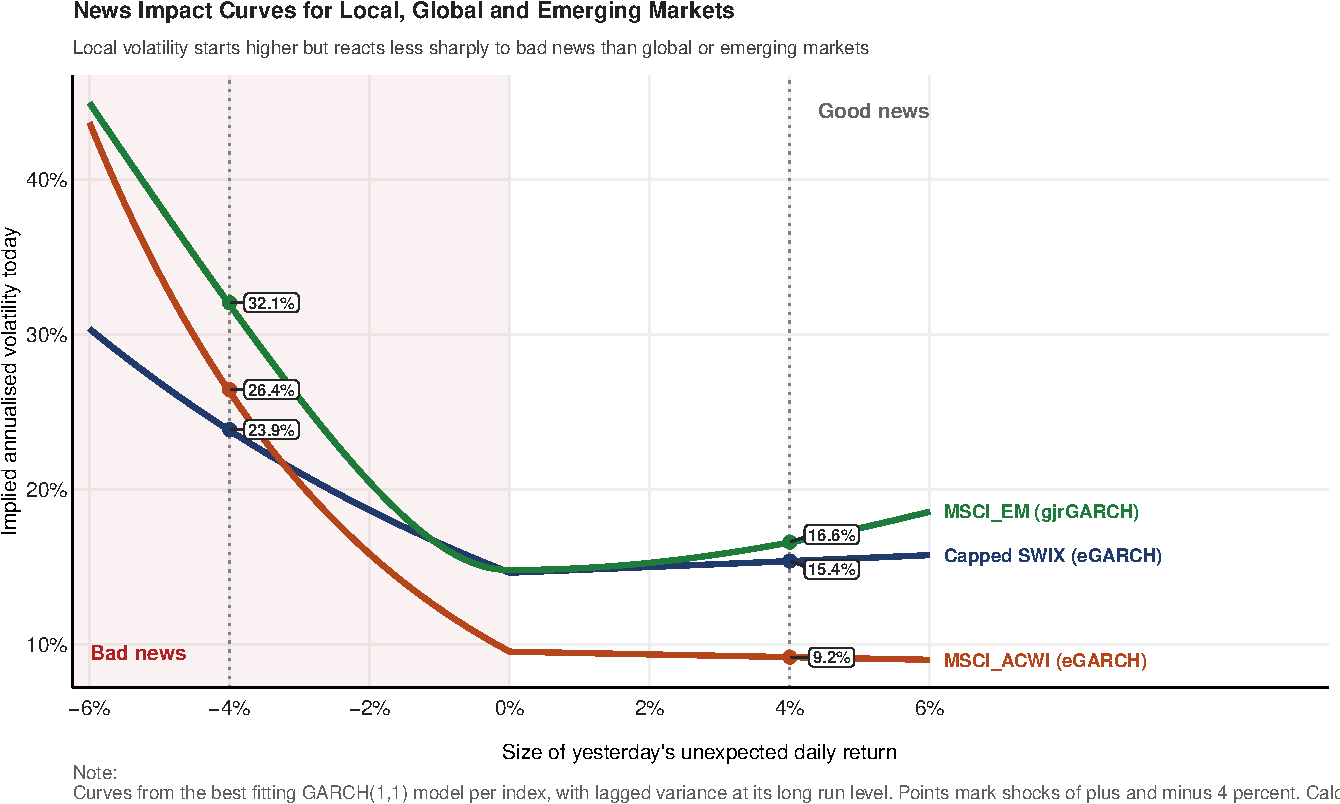
\includegraphics[width=1\linewidth]{Question1_files/figure-latex/q1a_nic-1} 

}

\caption{News Impact Curves for Local, Global and Emerging Markets}\label{fig:q1a_nic}
\end{figure}

Figure \ref{fig:q1a_nic} traces the news impact curve of each model. All
three rise more steeply after bad news, but the local curve is flatter,
with an asymmetry ratio of 1.55 against 2.87 globally. The local market
starts from a higher base but reacts less violently to falls, possibly
because of the weight of rand hedge shares.

\subsection{Forecasting Volatility
Forward}\label{forecasting-volatility-forward}

A GARCH model also says how long a volatility episode should last. The
selected model for each index is used to forecast conditional volatility
six months beyond the end of the sample, and the forecast is drawn next
to the recent fitted path and the long run level to which it converges.

\begin{figure}[H]

{\centering 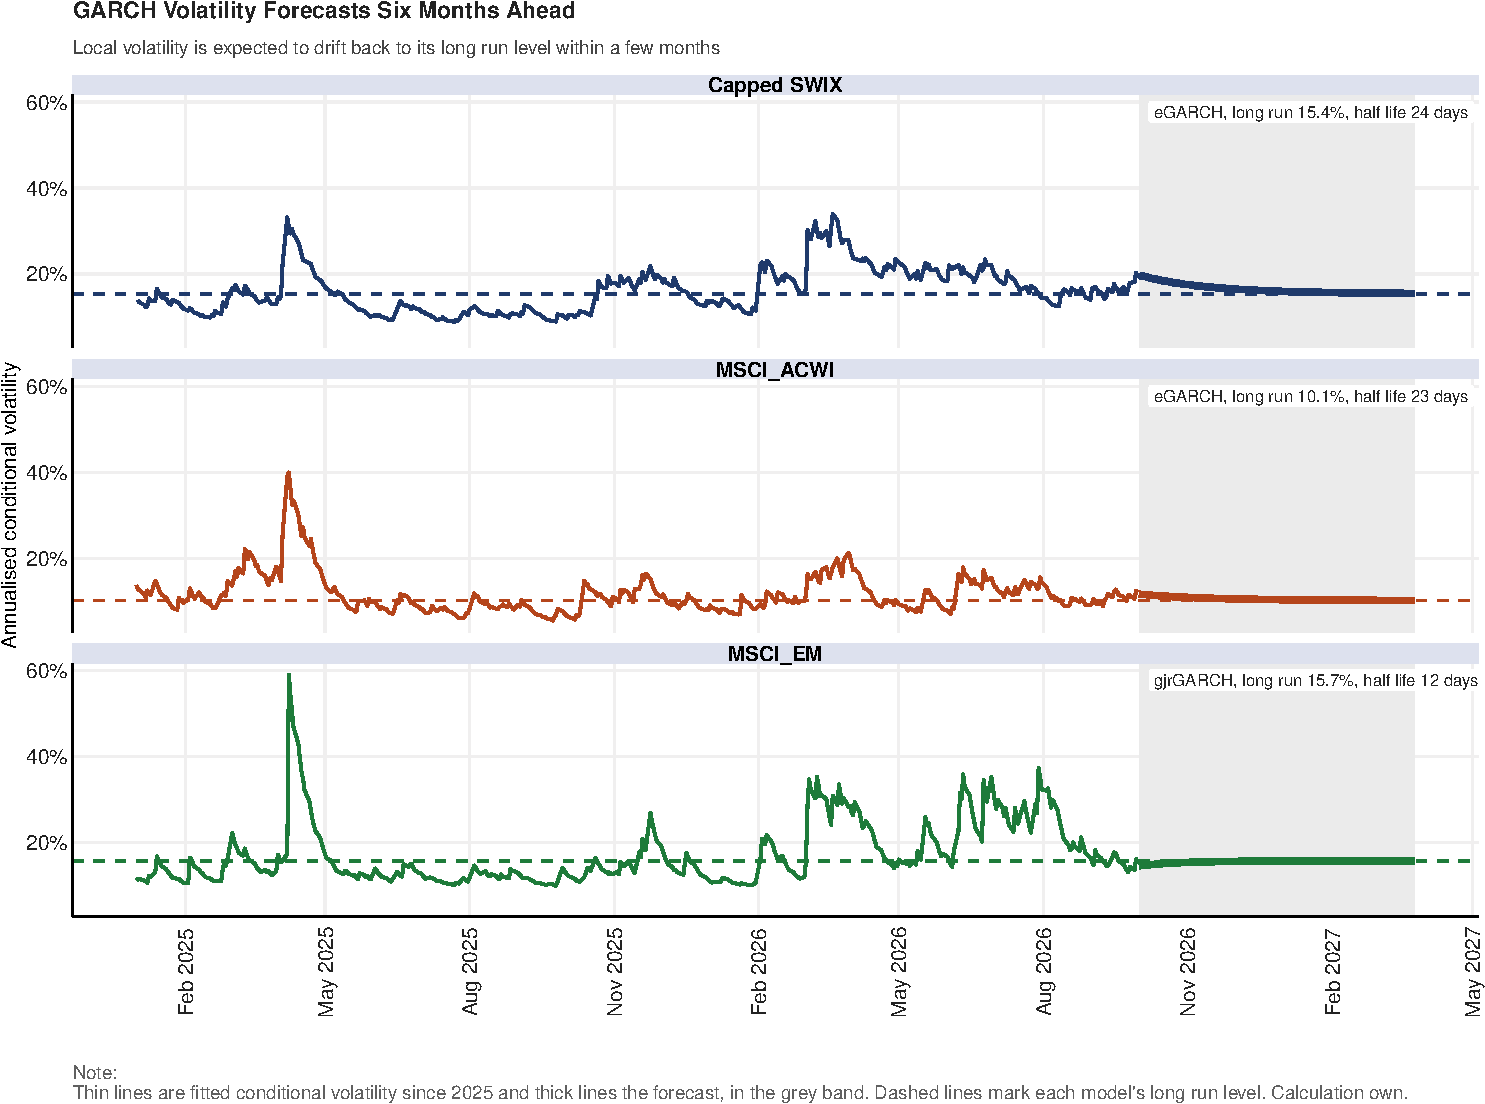
\includegraphics[width=1\linewidth]{Question1_files/figure-latex/q1a_forecast-1} 

}

\caption{GARCH Volatility Forecasts Six Months Ahead}\label{fig:q1a_forecast}
\end{figure}

The forecasts treat the 2026 episode as temporary. At the end of
September 2026 the conditional volatility of the Capped SWIX stood at
19.2 percent, above its long run level of 15.4 percent, and the model
projects it to fall to 16.0 percent within three months, since half of
any shock fades within about 24 trading days. Global volatility, at 12.1
percent, sits close to its long run level of 10.1 percent. Emerging
market volatility, whose shocks halve in only 12 days, had already
returned to its long run level of 15.7 percent by the end of the sample.
One qualification applies. A GARCH forecast always converges to the
average of the estimation sample, so it cannot detect a lasting shift in
the level of volatility, and the evidence against such a shift comes
from the rolling and heatmap results above.

\subsection{Co-movement with Global
Markets}\label{co-movement-with-global-markets}

Volatility can rise relative to global markets in two different ways.
The local market may become more tightly linked to them, so that global
shocks pass through more fully, or it may simply be exposed to larger
shocks in the markets it already moves with. The two carry different
implications for a risk ballast, so the time-varying correlation between
the Capped SWIX and the two MSCI indexes is estimated with a DCC model.
Weekly log returns are used because the Johannesburg and New York
markets close at different times, which biases daily correlations
downwards, and because log returns can be summed across the days of a
week. The lollipop chart shows each month's average correlation measured
from the pair's long run average, so that months of tighter co-movement
point up in red and months of looser co-movement point down in blue.

\begin{figure}[H]

{\centering 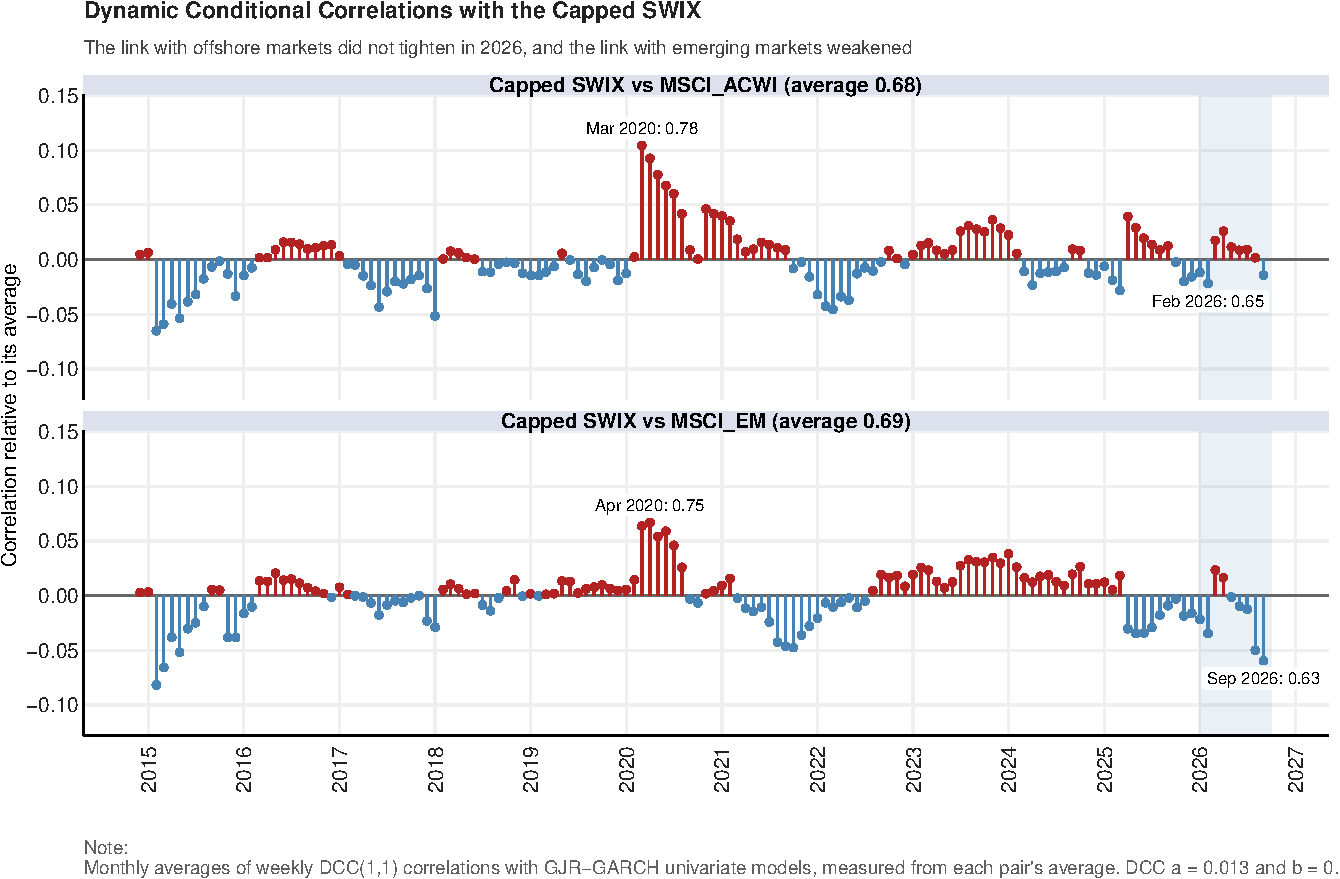
\includegraphics[width=1\linewidth]{Question1_files/figure-latex/q1a_dcc-1} 

}

\caption{Dynamic Conditional Correlations with the Capped SWIX}\label{fig:q1a_dcc}
\end{figure}

The correlations are stable, as the small size of most lollipops shows.
The local index has averaged a correlation of 0.68 with the global index
and 0.69 with emerging markets, and the fitted DCC parameters in the
caption imply that correlations adjust only slowly to new shocks. The
one clear break is the Covid crash, when the monthly correlation with
the global index rose to 0.78. In 2026 the correlation with the global
index averaged 0.68, almost unchanged from its 2021 to 2024 average of
0.68, while the correlation with emerging markets fell from 0.69 to 0.67
and reached 0.62 in August 2026, its lowest weekly reading since 2016.
The rise in local volatility therefore did not come from a tighter link
with offshore markets. It came instead from larger shocks to the
emerging market and commodity complex to which the local market is
exposed, and the run of blue lollipops in the second half of 2026
matches the heatmap, in which emerging market volatility kept rising
after local volatility had settled.

\subsection{Volatility Across Global
Regimes}\label{volatility-across-global-regimes}

The seminar attributed rising local volatility to oil price volatility
and global policy uncertainty. This claim is tested by stratifying the
sample. Each month is ranked by a state variable, and the top and bottom
quintiles of months are labelled stressed and calm. The volatility of
the Capped SWIX within those months is then compared with its full
sample volatility. Five state variables are considered, namely US and
emerging market implied volatility, rand volatility, the global economic
policy uncertainty index, and the realised volatility of Brent oil. The
dumbbell chart places each state's calm and stressed readings on one
line, with the gap between them in the column on the right.

\begin{figure}[H]

{\centering 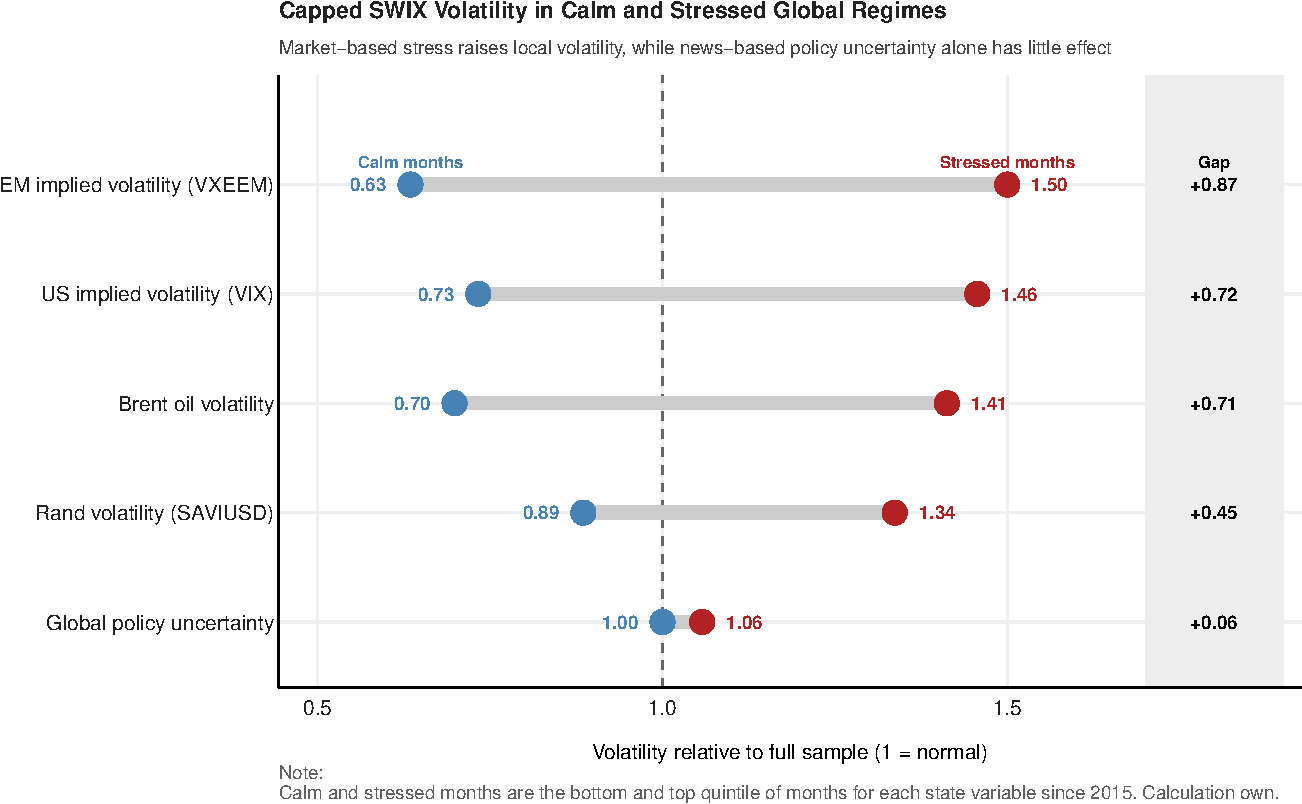
\includegraphics[width=1\linewidth]{Question1_files/figure-latex/q1a_stratify-1} 

}

\caption{Capped SWIX Volatility in Calm and Stressed Global Regimes}\label{fig:q1a_stratify}
\end{figure}

The chart separates market-based stress from news-based uncertainty. In
months when oil volatility sits in its top quintile, the Capped SWIX is
1.41 times as volatile as normal, and the equivalent ratios for emerging
market and US implied volatility are 1.50 and 1.46. Rand volatility has
a similar but smaller effect, at 1.34. Global policy uncertainty is the
exception, with a gap of only 0.06 between its calm and stressed months,
so the most uncertain months are barely more volatile than the calmest.
Policy uncertainty reached its highest annual average since 2015 in
2025, at 394 against 298 during the Covid year, yet it appears to affect
local share prices only once it is transmitted through a market channel,
such as oil prices or emerging market risk appetite.

\subsection{Volatility Across Local Size
Segments}\label{volatility-across-local-size-segments}

\begin{figure}[H]

{\centering 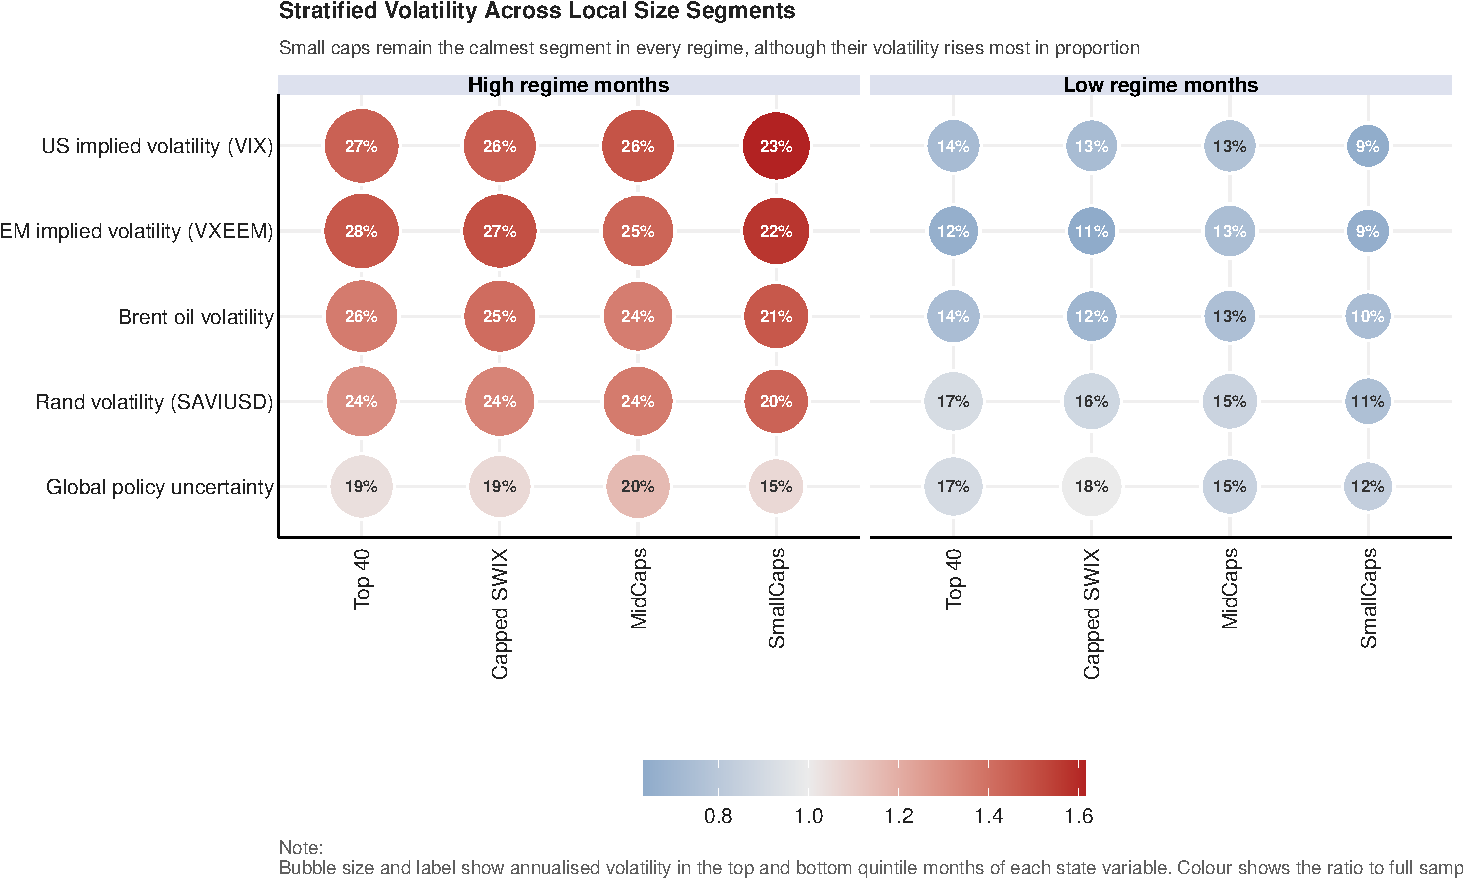
\includegraphics[width=1\linewidth]{Question1_files/figure-latex/q1a_size_bubbles-1} 

}

\caption{Stratified Volatility Across Local Size Segments}\label{fig:q1a_size_bubbles}
\end{figure}

Figure \ref{fig:q1a_size_bubbles} repeats the stratification across the
size indexes. Small caps are the calmest segment in every regime,
although their volatility rises most in proportion, up to 1.61 times
normal. Part of their calm may reflect stale prices in thinly traded
shares.

\subsection{Summary of Part A}\label{summary-of-part-a}

Local volatility has increased, subject to three qualifications. The
increase took the form of an episode, peaking in March and April 2026
and subsiding by the third quarter, and not as a permanent rise in the
level of volatility. It did not mirror the global experience, since
developed market volatility stayed below its average throughout 2026,
and instead followed emerging markets and the oil market. It also did
not reflect a tighter link with offshore markets, as the correlation
with global equities was little changed in 2026 and the correlation with
emerging markets fell. The local market reacts less sharply to bad news
than global markets do, which suggests a degree of built-in resilience.

For a team considering a risk ballast in a local fund, the relevant
threat is therefore a commodity and emerging market shock, more than a
developed market sell-off, and a ballast calibrated only to developed
market stress would have missed the 2026 episode. Within the local
market, small caps offer the best ballast in absolute terms, subject to
the liquidity caveat noted above. Part B examines whether SafeCore
already holds such a ballast.

\section{\texorpdfstring{Volatility and Factor Exposures of SafeCore
\label{PartB}}{Volatility and Factor Exposures of SafeCore }}\label{volatility-and-factor-exposures-of-safecore}

\subsection{Scope and Method}\label{scope-and-method-1}

This part evaluates whether SafeCore, a fund built without explicit
reference to volatility, has nonetheless managed volatility well. The
analysis has three strands. The first compares the fund's return and
risk profile with that of the Capped SWIX, its historical benchmark,
across the full sample, through time, and in the calm and stressed
regimes identified in Part A. The second decomposes the fund's
volatility into the contribution of each sector and stock, using
marginal contributions to risk. The third builds momentum and low
volatility scores from price behaviour, tests them against the vendor's
scores, and then uses all of the scores to compare SafeCore's factor
exposures with those of the local strategy indexes.

\subsection{Reconstructing the Fund and its
Benchmark}\label{reconstructing-the-fund-and-its-benchmark}

The rebuilt benchmark tracks the published J433 index closely, with
calendar year returns within one percentage point in 9 of the 12 years.

\subsection{Return and Risk Profile}\label{return-and-risk-profile}

The figure below sets out the return, risk and market capture measures,
calculated on monthly returns, over the full sample and since 2020.
Panel A tracks the fund's position in the up-market vs down-market
capture space relative to the benchmark at (1.00, 1.00), where points
below the diagonal line represent asymmetric alpha. Panel B contrasts
annualised return, volatility, max drawdown and tail risk across both
periods. The capture ratios use the arithmetic version of the
PerformanceAnalytics calculation, because the default geometric version
compounds every up or down month into a single return and overstates the
ratio.

\begin{figure}[H]

{\centering 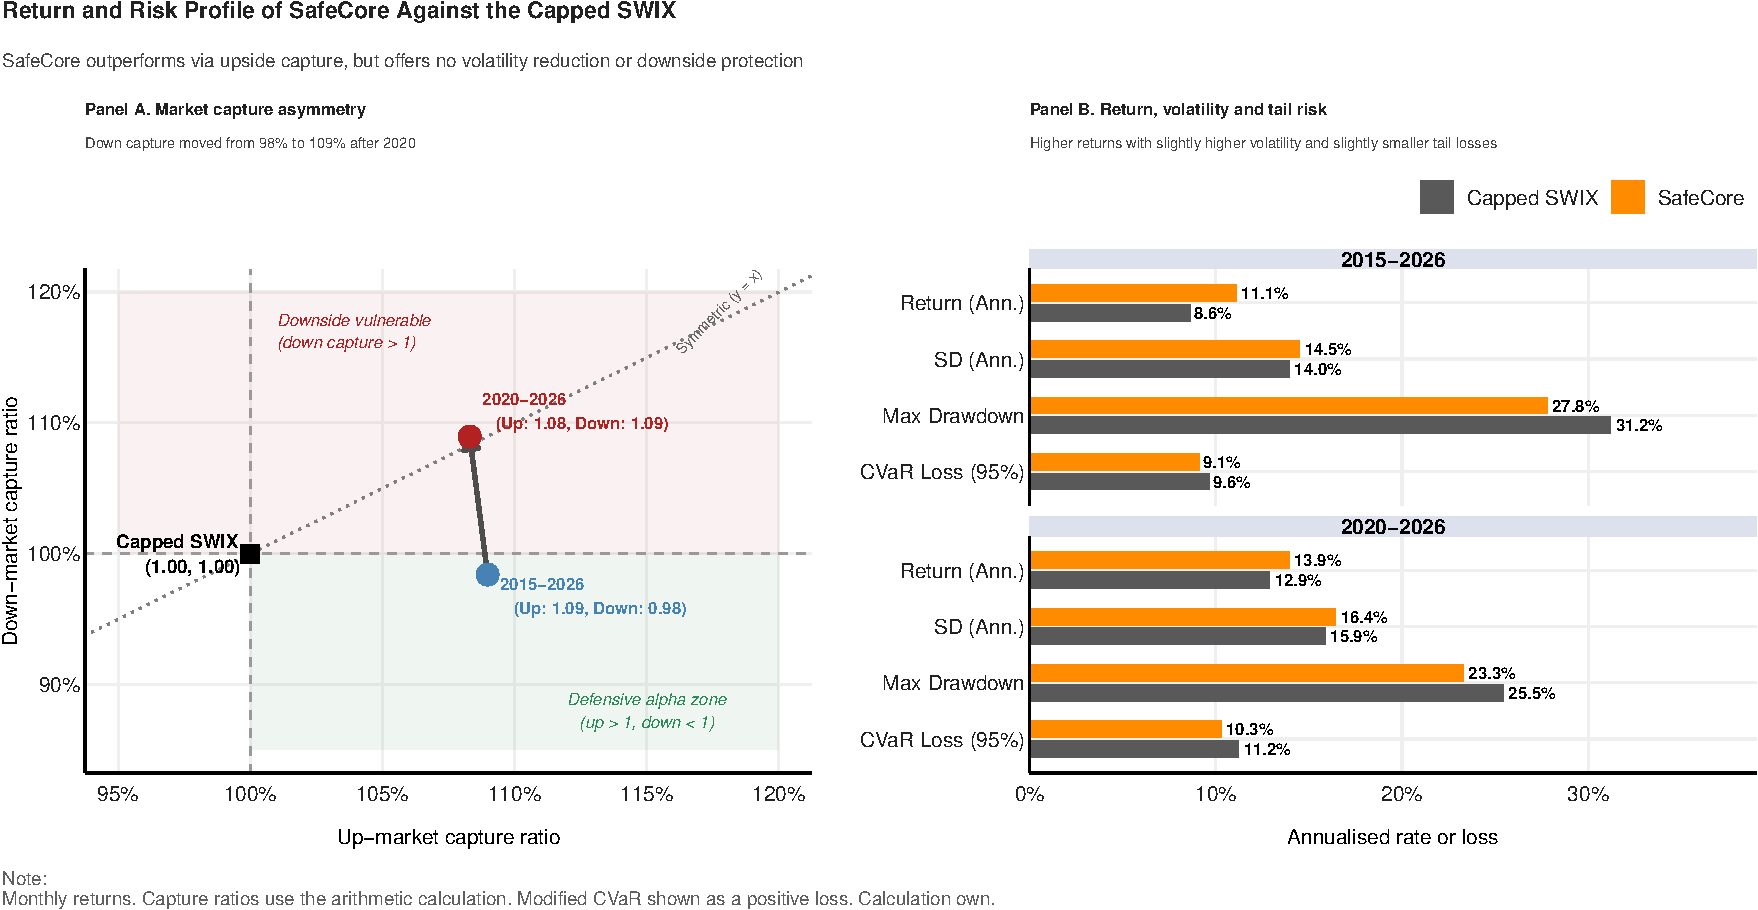
\includegraphics[width=1\linewidth]{Question1_files/figure-latex/q1b_capture-1} 

}

\caption{Return and Risk Profile of SafeCore Against the Capped SWIX}\label{fig:q1b_capture}
\end{figure}

SafeCore has delivered a better return than its benchmark, but it has
not done so by managing volatility. Over the full sample the fund
returned 10.9 percent a year against 8.4 percent, with an information
ratio of 0.62, yet its volatility of 14.6 percent was slightly higher
than the benchmark's 14.0 percent. Its beta of 1.00 shows that it moves
one for one with the market, and its down capture of 0.98 means that it
suffered almost the full extent of the benchmark's losses in falling
months. The fund's protective features are modest. Its maximum drawdown
of 27.9 percent was shallower than the benchmark's 31.7 percent, and its
modified CVaR was marginally lower. The outperformance therefore came
from stock selection in rising markets, with an up capture of 1.09, and
not from protection in falling ones. The more recent period is less
flattering still. Since 2020 the fund's down capture has risen to 1.09,
so it has lost more than the benchmark in falling months, and its
information ratio has fallen to 0.27.

\subsection{Daily Tail Risk}\label{daily-tail-risk}

\begin{figure}[H]

{\centering 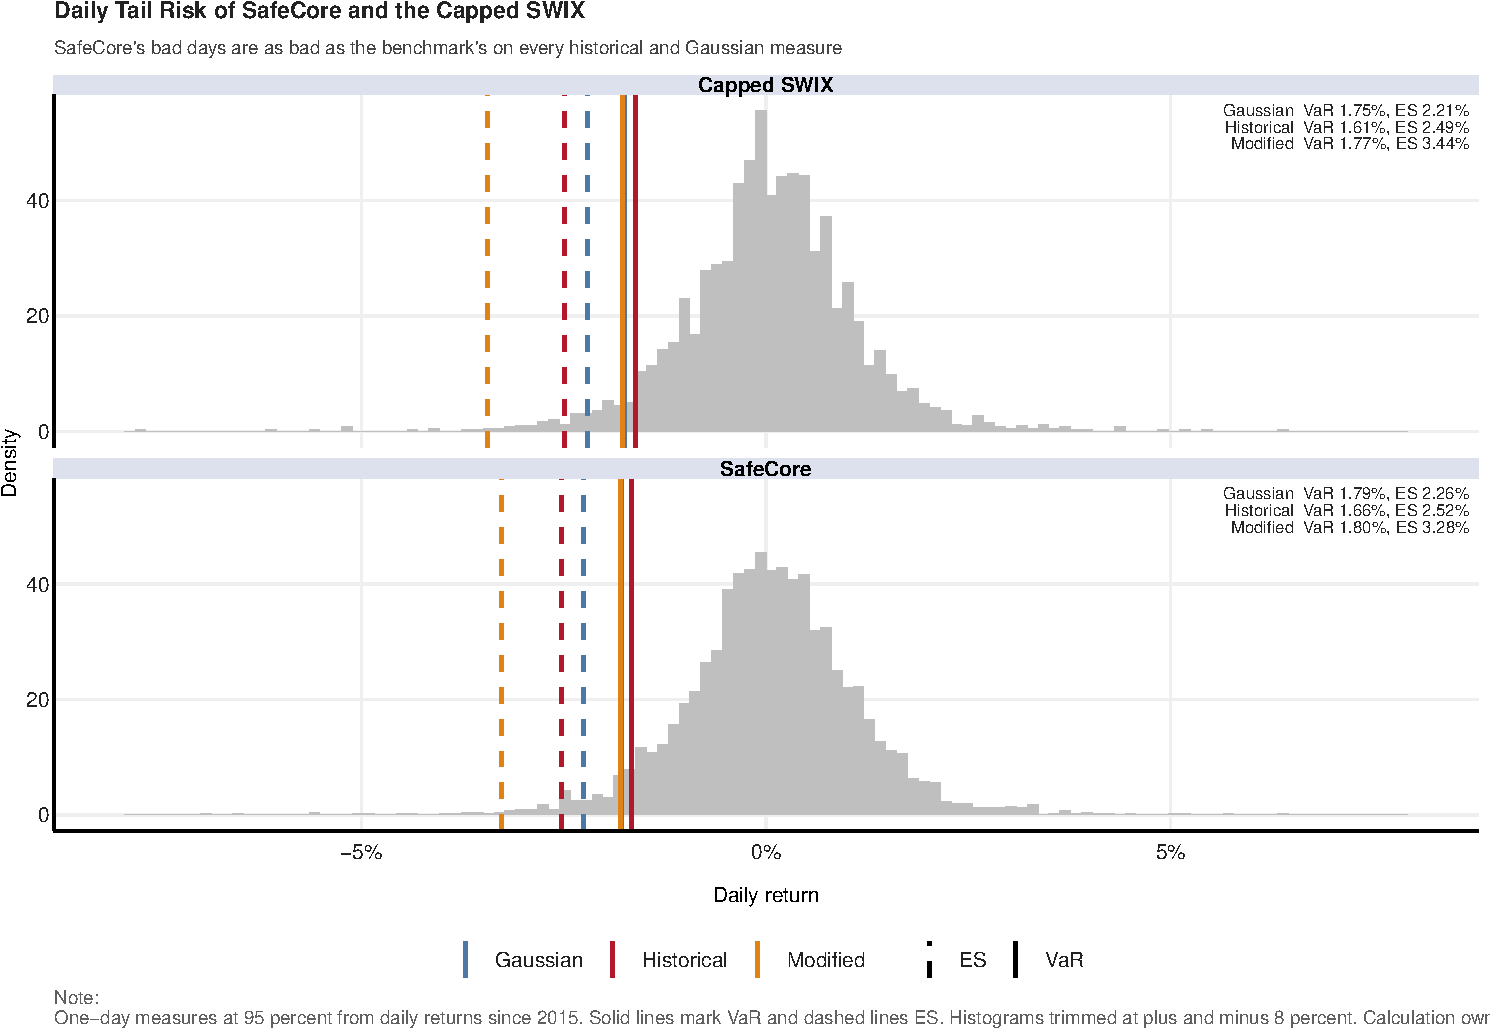
\includegraphics[width=1\linewidth]{Question1_files/figure-latex/q1b_tail-1} 

}

\caption{Daily Tail Risk of SafeCore and the Capped SWIX}\label{fig:q1b_tail}
\end{figure}

Figure \ref{fig:q1b_tail} compares one-day Value at Risk and Expected
Shortfall at 95 percent. The historical VaR is 1.66 percent for SafeCore
against 1.61 percent for the benchmark, and the historical ES is 2.52
percent against 2.49 percent. The fund's bad days are as bad as the
benchmark's.

\subsection{Calendar Year Returns}\label{calendar-year-returns}

\begin{figure}[H]

{\centering 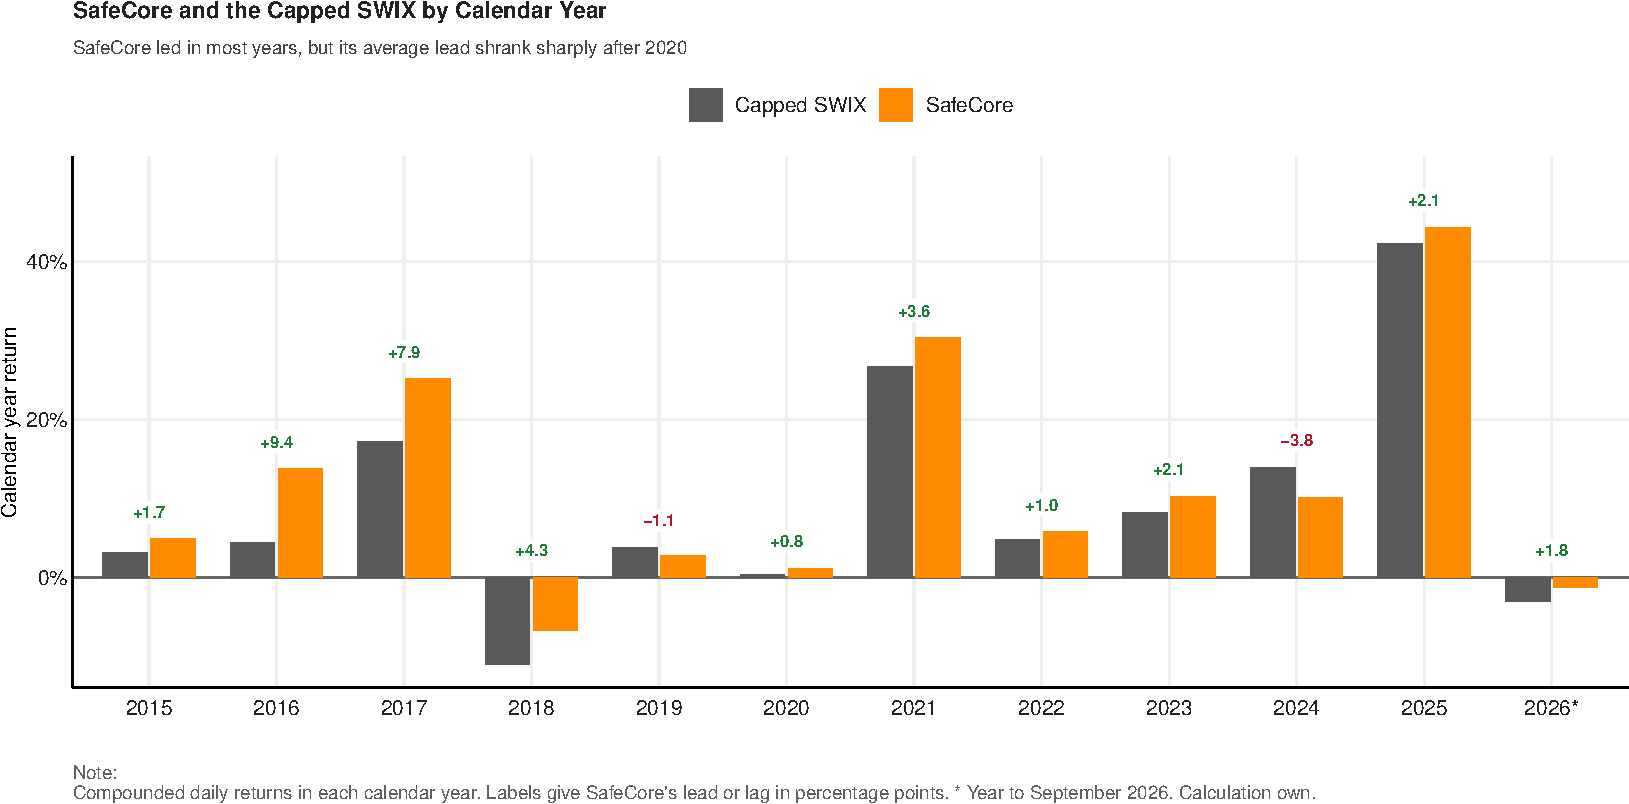
\includegraphics[width=1\linewidth]{Question1_files/figure-latex/q1b_calendar-1} 

}

\caption{SafeCore and the Capped SWIX by Calendar Year}\label{fig:q1b_calendar}
\end{figure}

Figure \ref{fig:q1b_calendar} shows that SafeCore beat its benchmark in
10 of 12 calendar years. Its average lead fell from 4.5 percentage
points a year in 2015 to 2019 to 1.0 points in 2020 to 2025.

\subsection{Rolling Volatility Relative to the
Benchmark}\label{rolling-volatility-relative-to-the-benchmark}

A full sample average can hide periods when the fund ran materially more
or less risk than the benchmark. The upper panel compares one year
rolling volatility, shading the space between the two lines red where
SafeCore was more volatile and blue where it was calmer, and the strip
underneath isolates the gap itself.

\begin{figure}[H]

{\centering 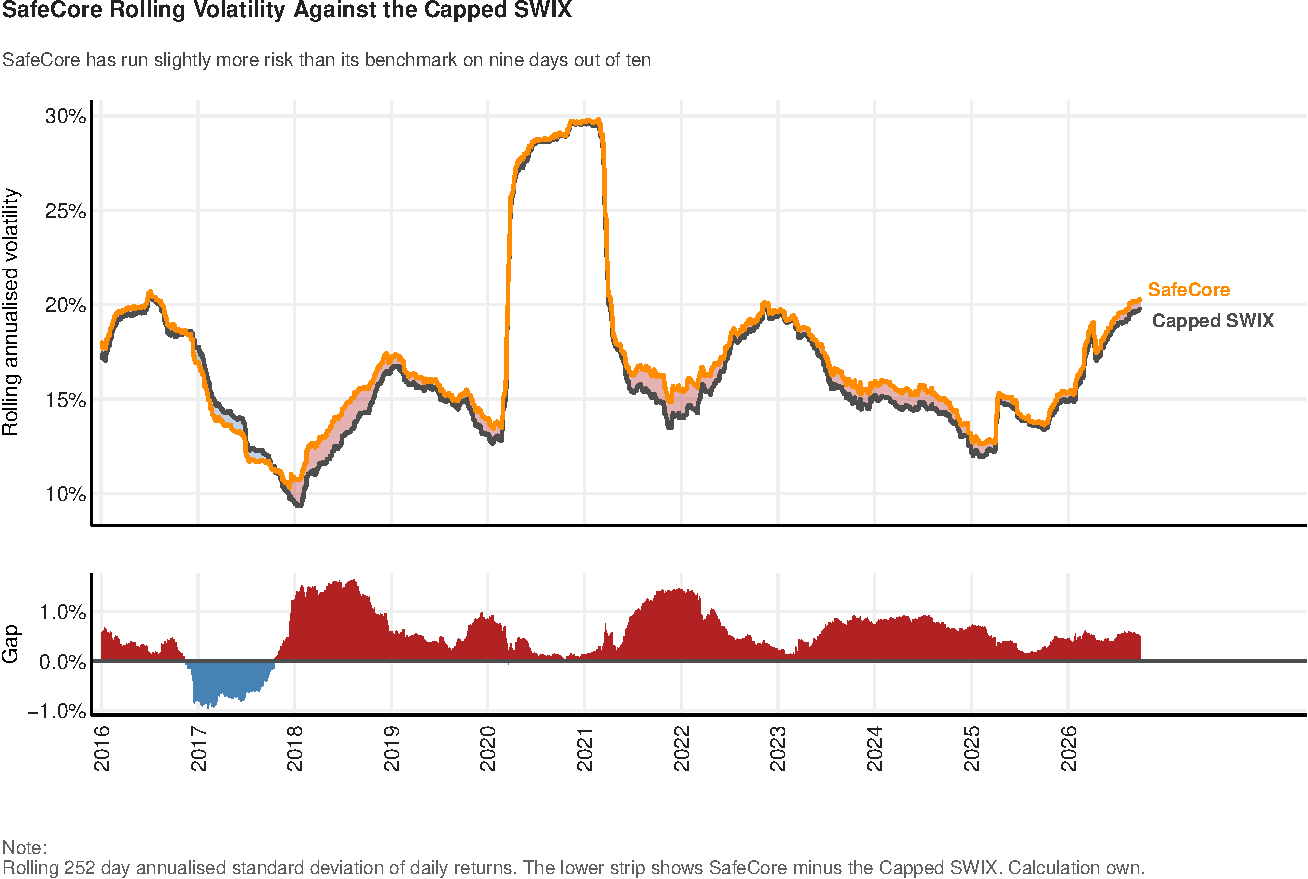
\includegraphics[width=1\linewidth]{Question1_files/figure-latex/q1b_rolling-1} 

}

\caption{SafeCore Rolling Volatility Against the Capped SWIX}\label{fig:q1b_rolling}
\end{figure}

The figure shows that SafeCore's excess volatility is persistent, and
not confined to a few episodes. The gap strip is red on 91 percent of
days since the rolling window begins in 2016, by an average of 0.5
percentage points, and it widened again from late 2025 as rolling
volatility for both rose towards 20 percent. The only sustained blue
stretch, in which SafeCore was calmer, came in 2017. The gap is small in
absolute terms, but it is persistent, and a fund that managed volatility
deliberately would be expected to sit below its benchmark at least some
of the time.

A ballast should also earn its keep when markets are stressed, so the
stratification from Part A is repeated for SafeCore and its benchmark.

In the stressed months of every state variable, SafeCore's volatility is
between 1.00 and 1.02 times the benchmark's, while in calm months it is
between 2 percent and 9 percent more volatile. SafeCore therefore adds
risk when markets are quiet and simply matches the market when they are
not, which is the opposite of the profile the seminar recommended.

\subsection{Sources of Portfolio
Volatility}\label{sources-of-portfolio-volatility}

The next question is where SafeCore's volatility comes from. On each
quarter end since 2015, the fund's volatility is decomposed into the
contribution of each holding, using the trailing year of daily returns.
Each stock's contribution is its weight multiplied by its marginal
contribution to risk, which captures both its own volatility and its
covariance with the rest of the fund, so that the contributions sum
exactly to the fund's total volatility. The mirrored area chart below
stacks each sector's share of capital above the axis and its share of
risk below it, so that any sector whose risk outgrows its capital shows
up as a band that is thicker underneath than on top.

\begin{figure}[H]

{\centering 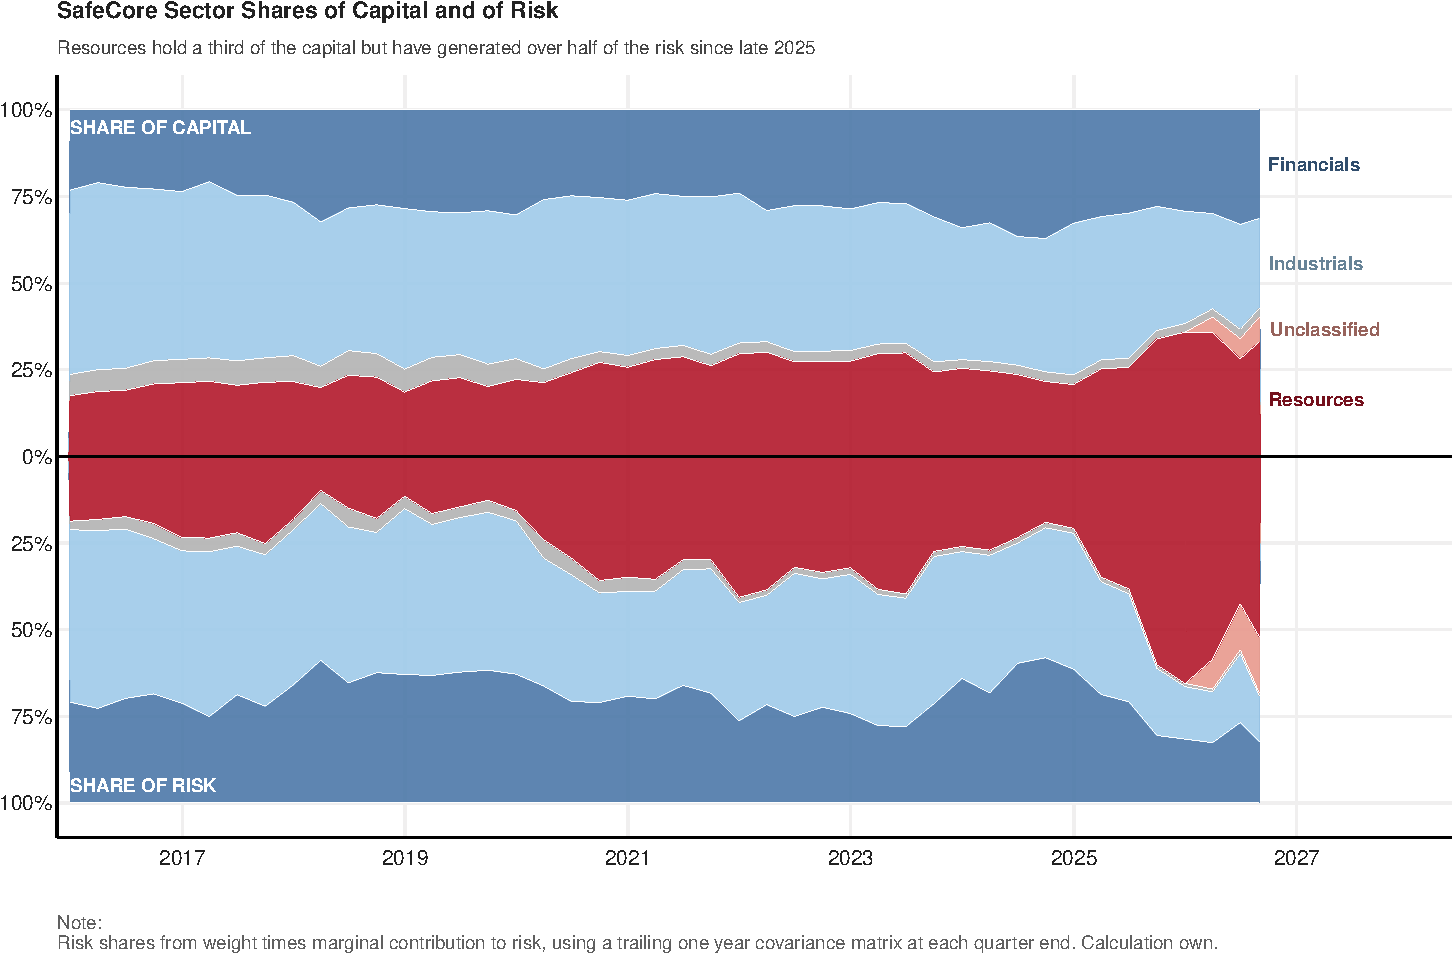
\includegraphics[width=1\linewidth]{Question1_files/figure-latex/q1b_risk-1} 

}

\caption{SafeCore Sector Shares of Capital and of Risk}\label{fig:q1b_risk}
\end{figure}

The chart shows a sharp change in where the fund's risk sits. Until 2024
the two halves broadly mirror each other, with financials taking a
somewhat larger share of risk than of capital, at 39 percent against 33
percent at the end of 2024. From the second half of 2025 the red
resources band swells below the axis while barely changing above it. At
the end of 2025 resources made up 36 percent of the fund but generated
65 percent of its volatility, and at the latest holdings date the
figures were 33 percent and 52 percent. The two unclassified holdings,
VAL and PAN, add a further 16 percent of risk on 7 percent of capital,
and since they appear to be Valterra Platinum and Pan African Resources,
the true resource share of risk is closer to two thirds.

\subsection{The Largest Contributors to
Risk}\label{the-largest-contributors-to-risk}

\begin{figure}[H]

{\centering 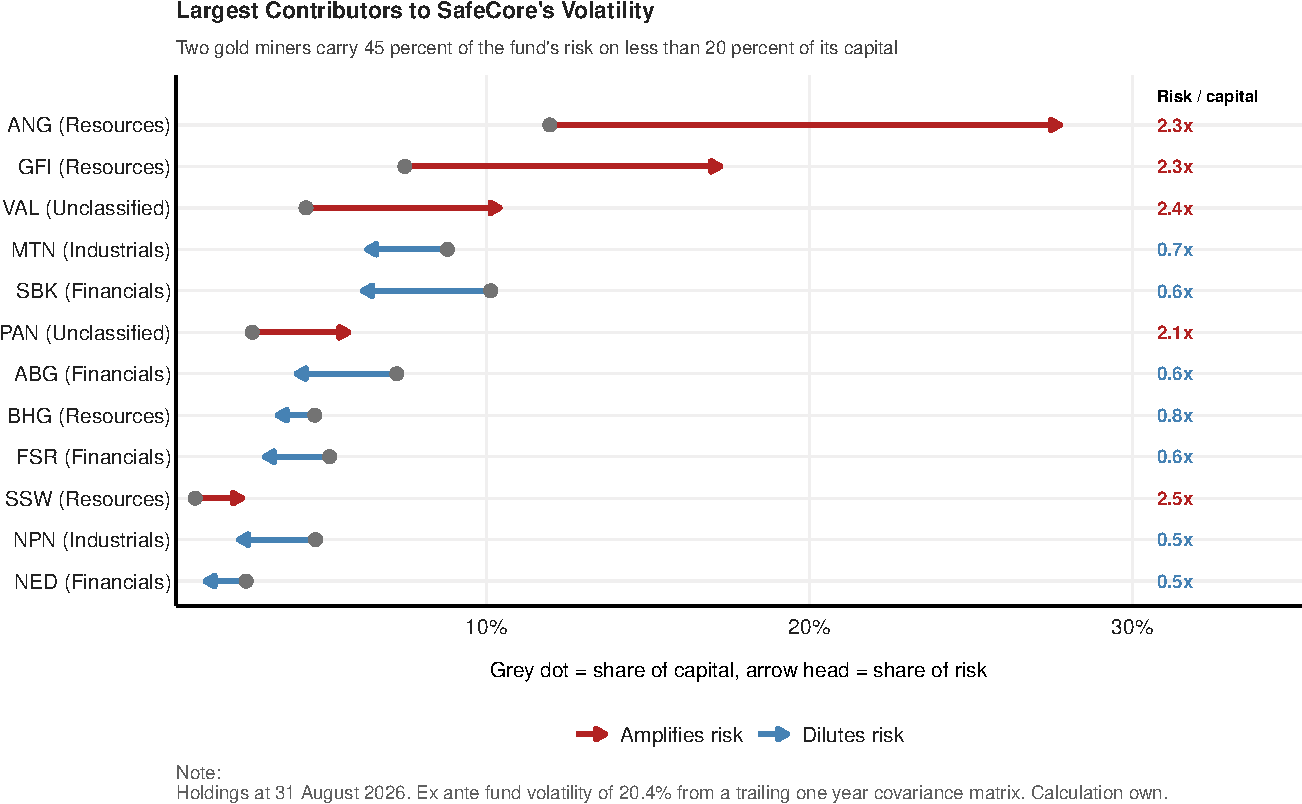
\includegraphics[width=1\linewidth]{Question1_files/figure-latex/q1b_top_risk-1} 

}

\caption{Largest Contributors to SafeCores Volatility}\label{fig:q1b_top_risk}
\end{figure}

Figure \ref{fig:q1b_top_risk} shows why. At the latest holdings date
AngloGold Ashanti and Gold Fields carried 45 percent of the fund's risk
on 19 percent of its capital, so the fund's volatility had become
largely a bet on the gold price.

\subsection{Building Own Momentum and Low Volatility
Scores}\label{building-own-momentum-and-low-volatility-scores}

Momentum is measured as the cumulative return from six months to one
month before each month end, following the suggestion in the paper.
Skipping the most recent month avoids the short term reversal effect, in
which last month's winners tend to give back part of their gains. A six
month window is preferred to the more common twelve month window because
it responds faster when market leadership rotates, which matters for a
fund concerned with volatility. The low volatility score is the negative
of each stock's annualised realised volatility over the past six months,
so that a higher score always indicates a more defensive stock. Realised
volatility is preferred to beta because SafeCore's concern is the total
volatility of its holdings, and because realised volatility is highly
persistent, which makes the recent past a reasonable guide to the near
future.

Both measures use daily returns capped at 25 percent and require a stock
to have traded on at least 80 percent of the days in the window. Each
month they are converted into cross-sectional z-scores within the
vendor's universe and winsorised at three standard deviations, which
places them on the same scale as the vendor's scores. A 12-1 momentum
score and each stock's market and downside beta are also calculated,
purely to diagnose what the vendor's scores measure.

\subsection{Own Scores Against the Vendor
Scores}\label{own-scores-against-the-vendor-scores}

The comparison uses the Spearman rank correlation across stocks each
month, since what matters for a factor portfolio is whether two scores
rank stocks in the same order, regardless of whether their values
coincide. The left panel tracks three comparisons through time, labelled
directly at the end of each line, while the heatmap on the right reports
the average rank correlation between every own measure and every vendor
factor, which shows what each vendor factor actually tracks.

\begin{figure}[H]

{\centering 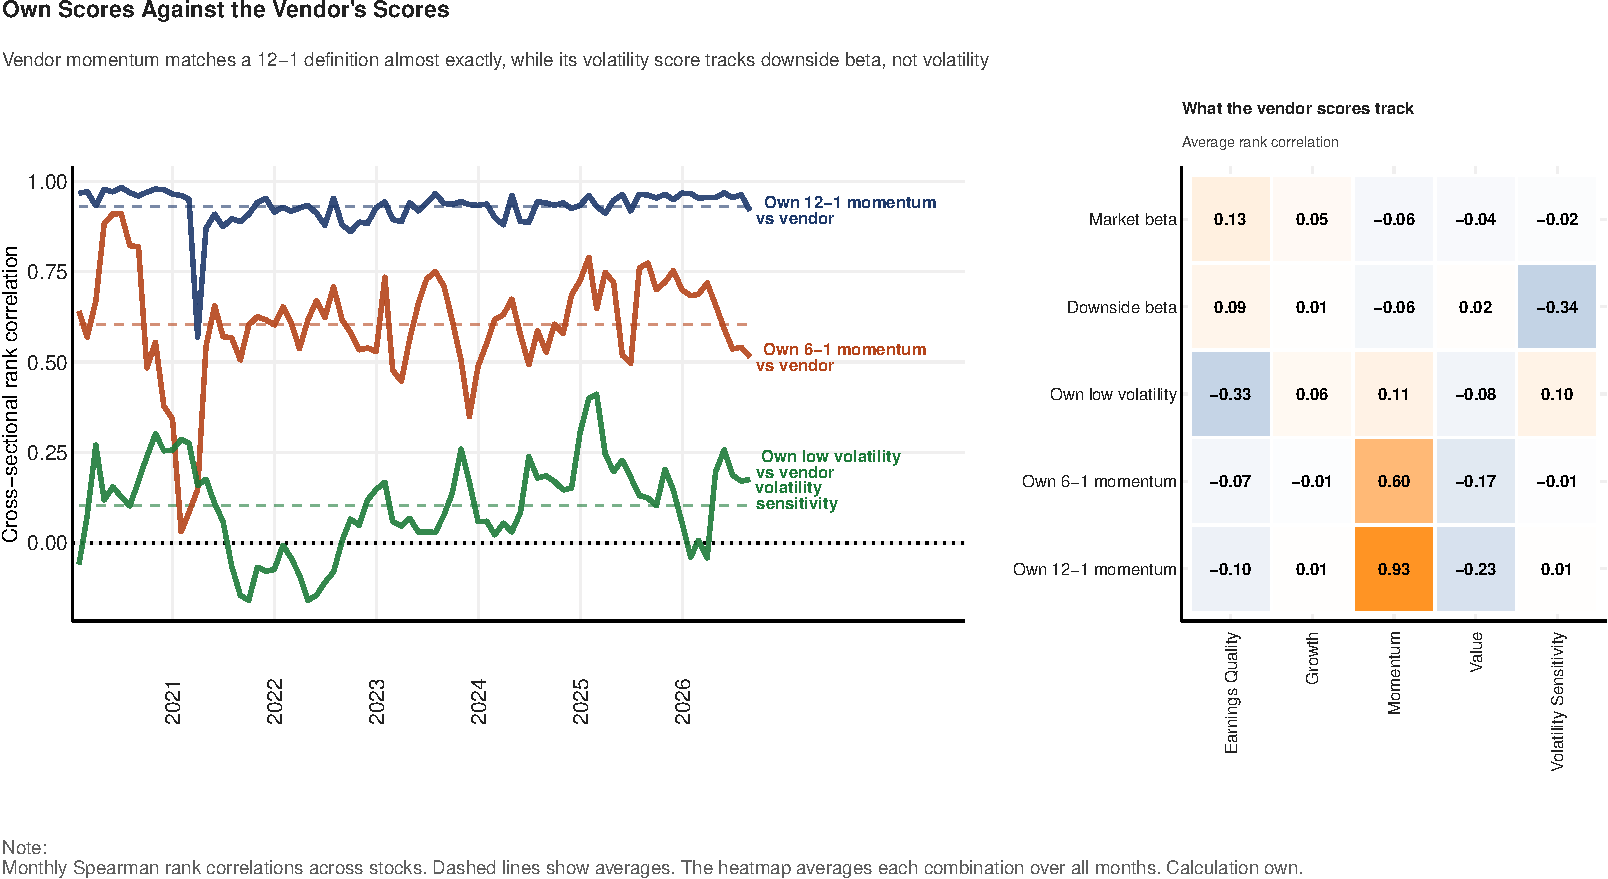
\includegraphics[width=1\linewidth]{Question1_files/figure-latex/q1b_score_compare-1} 

}

\caption{Own Scores Against the Vendors Scores}\label{fig:q1b_score_compare}
\end{figure}

The comparison yields two clear findings about the vendor's data. The
vendor's momentum score is almost certainly a 12-1 measure, since a 12-1
score built from prices ranks stocks the same way with an average
correlation of 0.93, while the 6-1 score proposed in the paper agrees
only at 0.60 and dropped close to zero in early 2021. The two momentum
scores therefore answer different questions, with the shorter window
capturing more recent shifts in leadership.

The vendor's volatility score is more problematic. It has an average
rank correlation of only 0.10 with the own low volatility score and fell
below zero for much of 2021 and 2022. The heatmap suggests what it
measures instead, since its strongest relationship is with downside
beta, at -0.34, meaning that stocks which fall most when the market
falls receive the lowest scores. Volatility Sensitivity is therefore
closer to a measure of downside market exposure than of total
volatility. A further oddity is that the vendor's earnings quality score
correlates at -0.33 with the own low volatility score, so the vendor
rates more volatile stocks as having higher quality earnings, which is
the opposite of what quality strategies usually assume. Both findings
counsel caution before using the vendor scores to steer a defensive
mandate.

\subsection{Composite Factor Scores Across
Strategies}\label{composite-factor-scores-across-strategies}

\begin{figure}[H]

{\centering 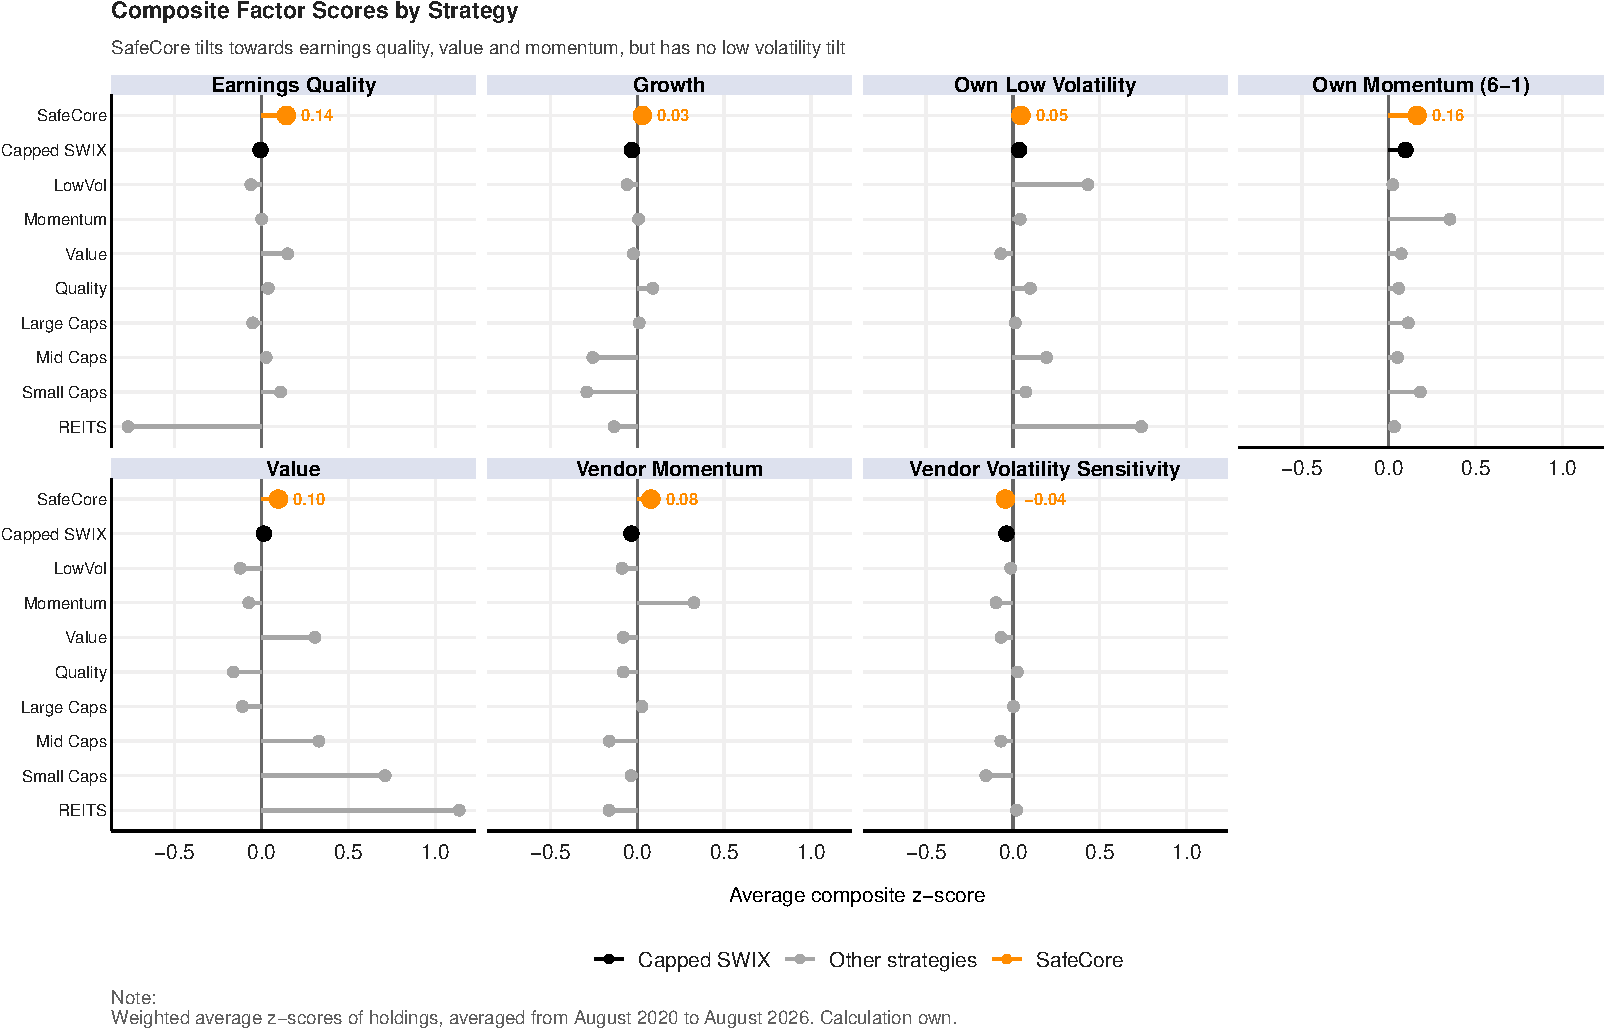
\includegraphics[width=1\linewidth]{Question1_files/figure-latex/q1b_composite-1} 

}

\caption{Composite Factor Scores by Strategy}\label{fig:q1b_composite}
\end{figure}

Figure \ref{fig:q1b_composite} shows holdings-weighted composite scores.
The own low volatility score identifies the LowVol index correctly, at
0.43 against 0.04 for the benchmark, while SafeCore tilts towards
quality, value and momentum but carries no low volatility tilt.

\subsection{SafeCore's Active Factor
Exposures}\label{safecores-active-factor-exposures}

\begin{figure}[H]

{\centering 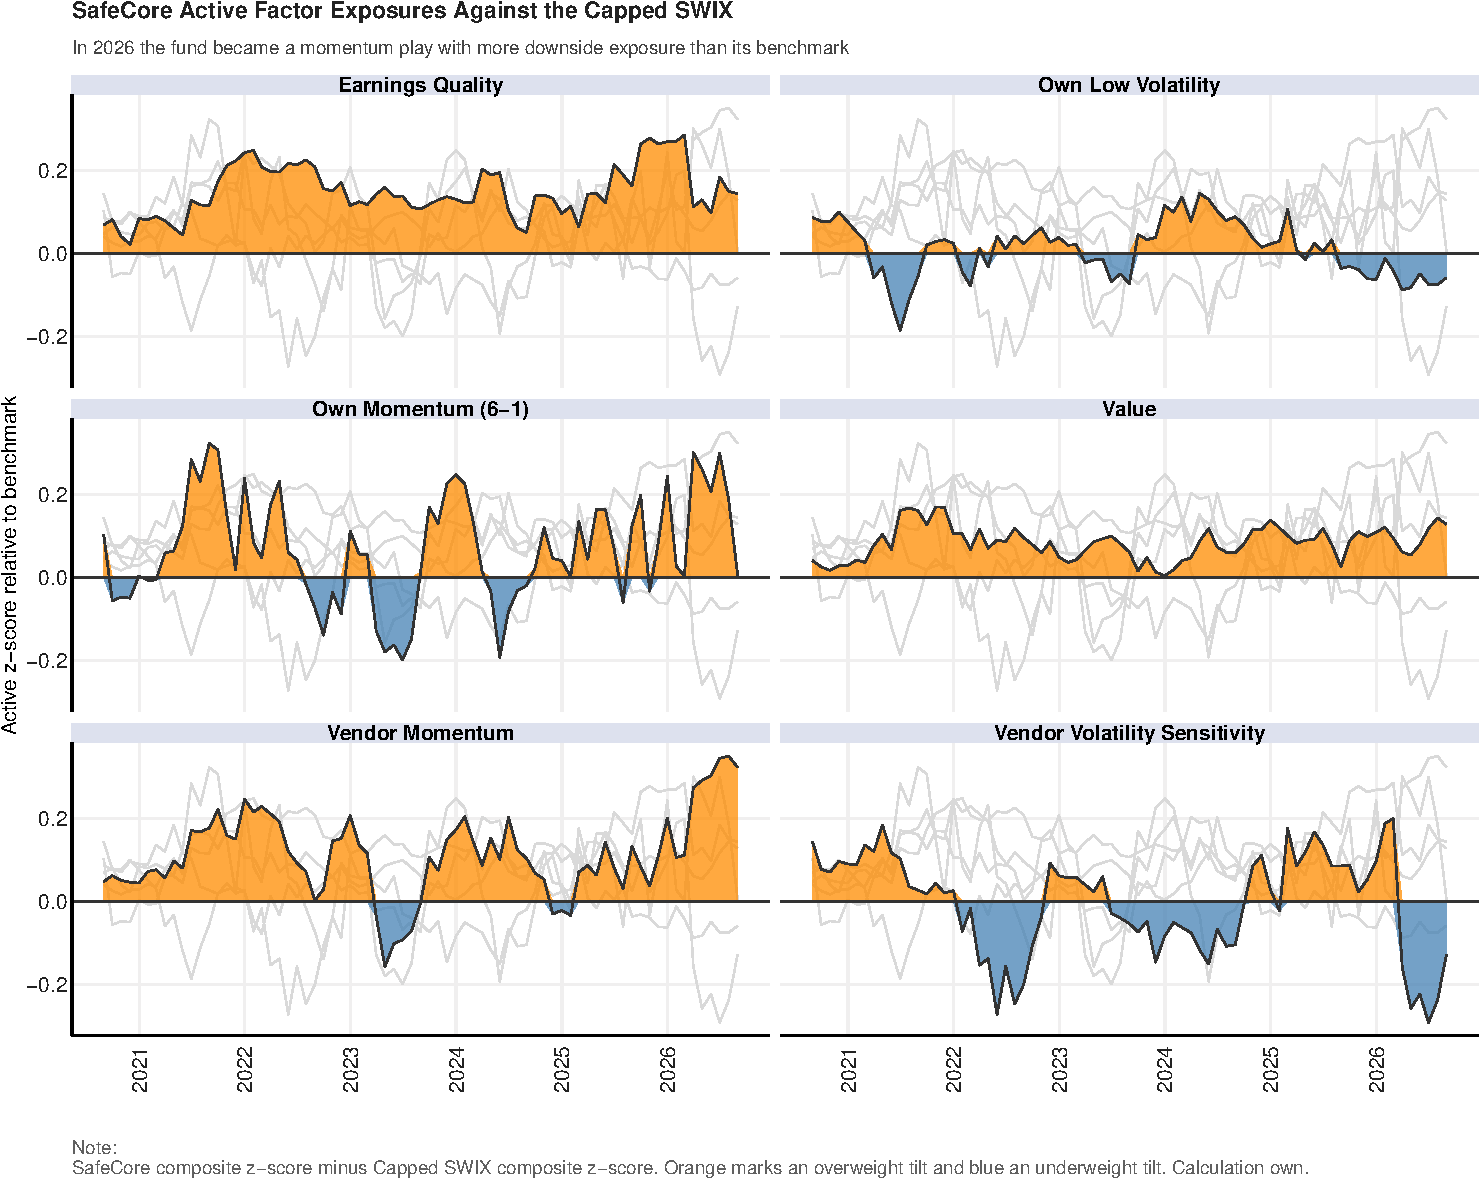
\includegraphics[width=1\linewidth]{Question1_files/figure-latex/q1b_active-1} 

}

\caption{SafeCore Active Factor Exposures Against the Capped SWIX}\label{fig:q1b_active}
\end{figure}

Figure \ref{fig:q1b_active} tracks active exposures through time. In
2026 the fund became a momentum play, with an active vendor momentum
exposure of 0.26 against 0.10 before 2025.

\subsection{Summary of Part B}\label{summary-of-part-b}

SafeCore does not navigate volatility effectively, although it has been
successful on other measures. The fund outperformed the Capped SWIX by
2.5 percentage points a year with an information ratio of 0.62, and its
drawdowns were somewhat shallower. That success came from stock
selection in rising markets, not from risk management. The fund has been
slightly more volatile than its benchmark on 91 percent of days, it
merely matches the benchmark's volatility in stressed regimes, it has
lost more than the benchmark in falling months since 2020, and it
carries no meaningful low volatility exposure. Its risk has also become
highly concentrated, with two gold miners generating 45 percent of the
fund's volatility at the latest holdings date.

For the team, three implications follow. The fund's risk is currently a
concentrated bet on precious metals, far from a broad equity exposure,
which the investment committee should either accept explicitly or
reduce. A low volatility sleeve or a cap on any single stock's
contribution to risk would be a more direct route to a risk ballast than
relying on the fund's existing quality and value tilts. Lastly, the
vendor's volatility score should not be used to build such a sleeve,
since it fails to identify the existing low volatility index, and a
score built from realised volatility does the job considerably better.

\section{\texorpdfstring{Dispersion, Correlation and Alpha Opportunity
\label{PartC}}{Dispersion, Correlation and Alpha Opportunity }}\label{dispersion-correlation-and-alpha-opportunity}

\subsection{Scope and Method}\label{scope-and-method-2}

This part measures the opportunity that the local market has offered
active managers since 2020 and how that opportunity has moved with the
global macro backdrop. Alpha opportunity is the scope for a manager's
portfolio to differ in outcome from the benchmark, and it depends on two
things. Stocks must move by different amounts, which is measured by
cross-sectional dispersion, and they must not all move together, which
is measured by inter-constituent correlation. The analysis therefore
measures both, shows how they combine, tests whether the opportunity
translated into different outcomes for South African active managers,
and finally relates both measures to global macro variables.

The analysis uses the daily constituents and weights of the Capped SWIX,
which start in August 2020 and so match the period the question asks
about. Daily constituent returns above 50 percent in absolute value are
winsorised, since the file contains a handful of implausible values.

\subsection{Cross-Sectional
Volatility}\label{cross-sectional-volatility}

Dispersion is measured as the cross-sectional volatility of each stock's
compounded return over a rolling 21 trading day window. The weighted
version follows the formula in the paper, weighting each stock's squared
deviation from the index return by its index weight, while the
unweighted version is the simple standard deviation across stocks. The
weighted measure is preferred as the headline, because an active manager
is measured against a cap-weighted benchmark. A large move in a
heavyweight stock forces every manager into a large active bet whether
they own the stock or not, while a large move in a stock that makes up
0.1 percent of the index barely matters. The unweighted measure is shown
for comparison, since it gives the same voice to small and illiquid
stocks whose returns are noisier.

\begin{figure}[H]

{\centering 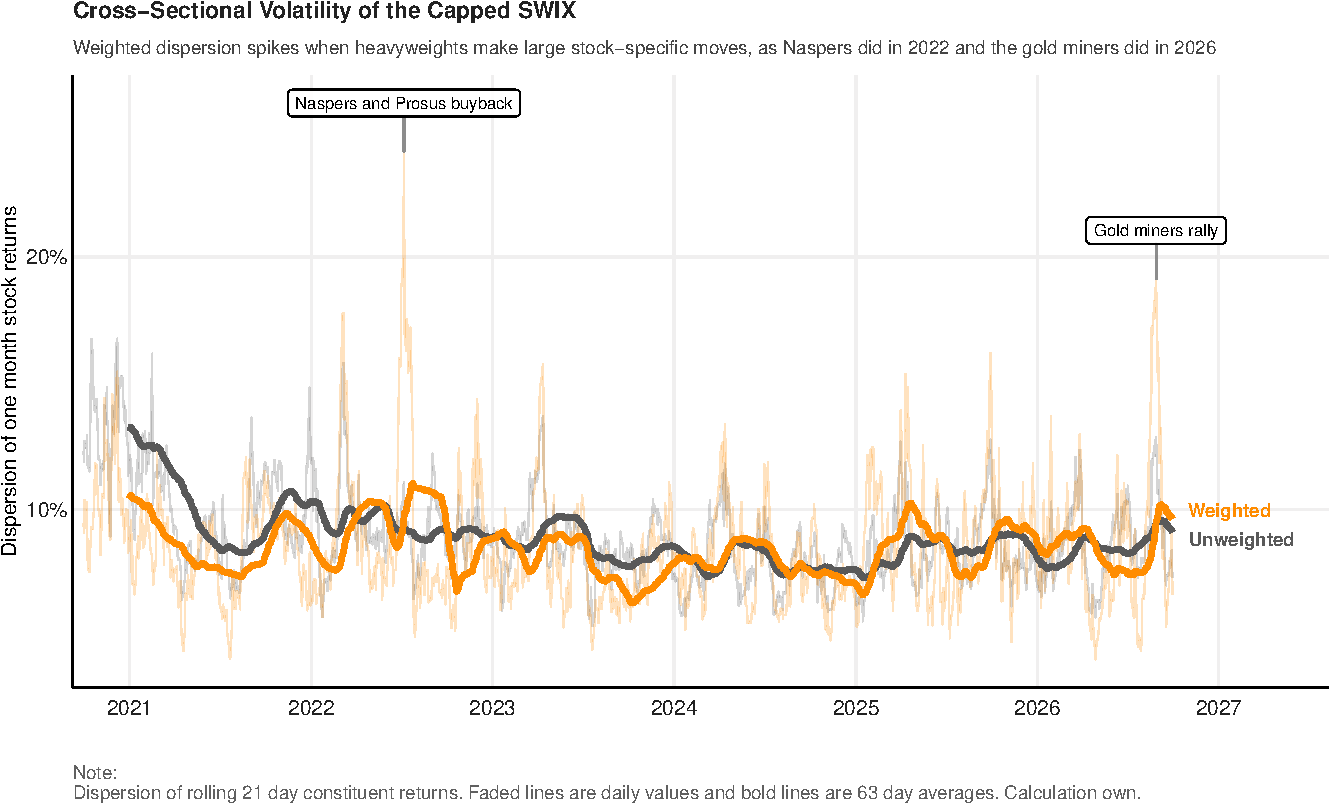
\includegraphics[width=1\linewidth]{Question1_files/figure-latex/q1c_dispersion-1} 

}

\caption{Cross-Sectional Volatility of the Capped SWIX}\label{fig:q1c_dispersion}
\end{figure}

The two measures tell different stories at the extremes. Weighted
dispersion averaged 8.5 percent before 2026 against 9.0 percent for the
unweighted measure, but its spikes are far sharper, reaching 24.1
percent in July 2022. Decomposing that spike stock by stock shows that
Naspers and Prosus alone account for most of it, after the two shares
rallied by more than 50 percent in a month on the announcement of an
open-ended share buyback. The second spike, in August 2026, came from
the gold miners, which gained around 40 percent in a month while the
index rose by less than 10 percent. These episodes show why the weighted
measure is the right one for this question. A manager who was
underweight Naspers in mid 2022 or underweight gold in 2026 faced a
large relative loss, and only the weighted measure registers that risk.
In 2026 weighted dispersion averaged 8.7 percent, close to its earlier
level, so the volatility episode of Part A did not translate into a
lasting rise in dispersion.

\subsection{Rolling Inter-Constituent
Correlation}\label{rolling-inter-constituent-correlation}

Correlation is measured over a rolling three month window at each month
end for the 40 largest constituents, which make up the bulk of the
index's weight. Two versions are calculated. The first is the simple
average of all pairwise correlations. The second is a cap-weighted
implied correlation, built along the lines of the CBOE implied
correlation index, which finds the single correlation that, applied to
every pair of stocks, reproduces the actual variance of the cap-weighted
basket. Because it weights pairs by the size of the stocks involved, the
gap between the two shows whether the largest stocks are moving together
more or less than the average pair.

\begin{figure}[H]

{\centering 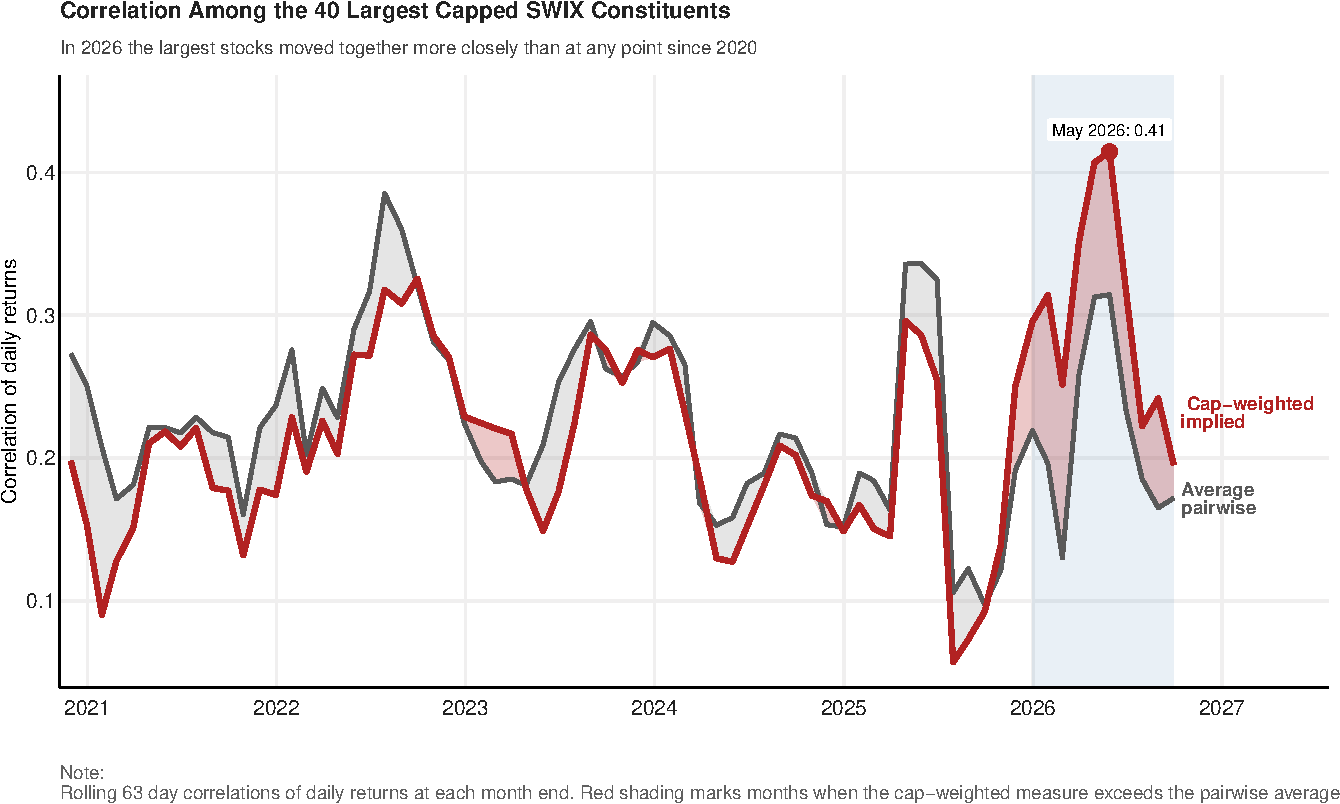
\includegraphics[width=1\linewidth]{Question1_files/figure-latex/q1c_correlation-1} 

}

\caption{Correlation Among the 40 Largest Capped SWIX Constituents}\label{fig:q1c_correlation}
\end{figure}

The implied correlation ranged from 0.06 to 0.41 over the sample, with
peaks in mid 2022 during global monetary tightening and in 2026. The
2026 peak is the larger of the two. The cap-weighted implied correlation
averaged 0.30 in 2026 against 0.20 before it, and for most of 2026 it
sat well above the simple pairwise average, which shows that the largest
stocks in particular were moving as a block. That pattern is consistent
with Part B, where the index's heaviest resource names drove a growing
share of risk. In mid 2025, by contrast, the implied correlation fell
below 0.1, the most favourable environment for stock pickers in the
sample.

\subsection{How Volatility and Correlation
Combine}\label{how-volatility-and-correlation-combine}

Dispersion and correlation are two sides of the same coin. The weighted
average variance of the constituents can be split exactly into the part
that is common to the basket, which no stock picker can avoid, and the
remainder, which is the weighted cross-sectional variance. The remainder
is the alpha opportunity, and its share of total stock risk is the
fraction of a stock's volatility that an active manager can actually
exploit.

\begin{figure}[H]

{\centering 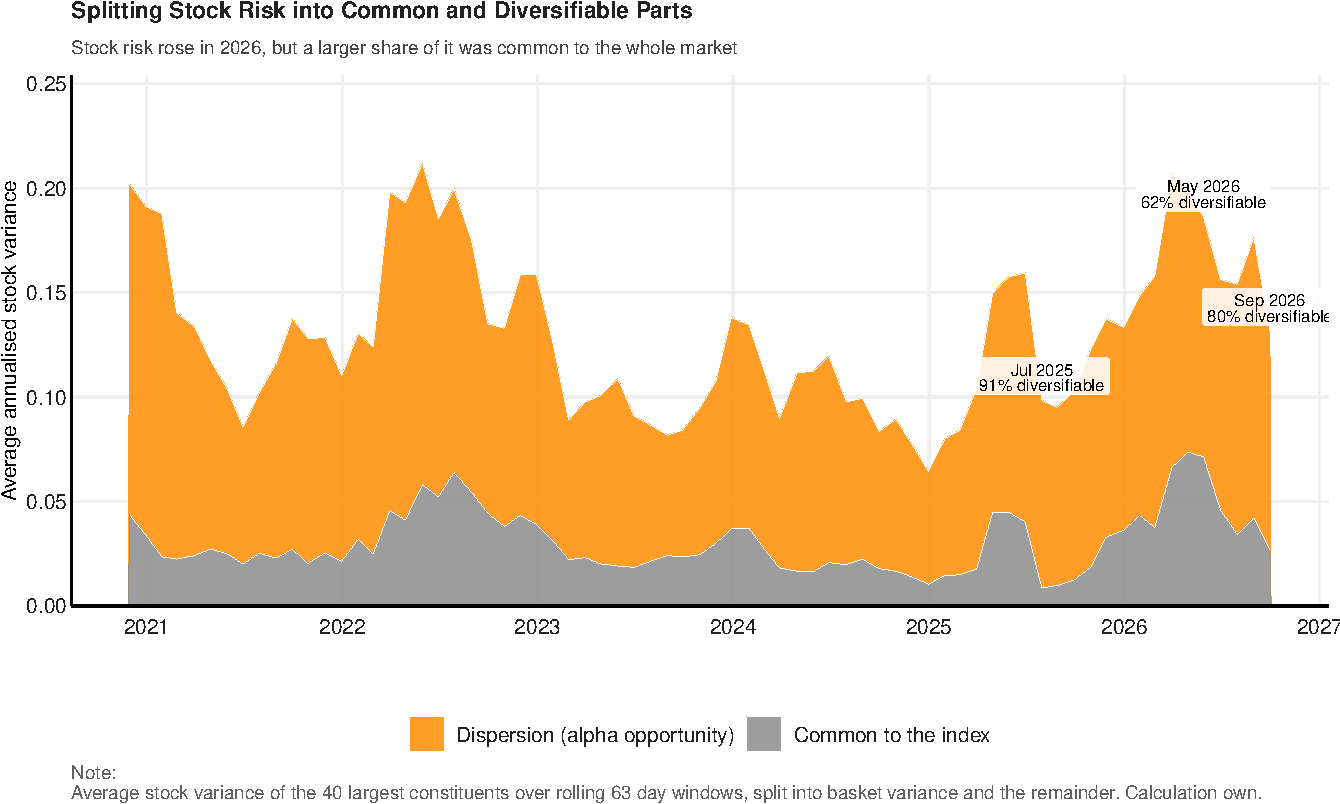
\includegraphics[width=1\linewidth]{Question1_files/figure-latex/q1c_split-1} 

}

\caption{Splitting Stock Risk into Common and Diversifiable Parts}\label{fig:q1c_split}
\end{figure}

The split shows that total stock risk and alpha opportunity do not
always move together. Average stock volatility rose to 37 percent in
2026 from 33 percent before it, yet the diversifiable share of that risk
fell from an average of 78 percent to 72 percent, reaching its lowest
point in May 2026. The orange band did widen in absolute terms, so there
was more raw dispersion to exploit, but much of the extra volatility was
common to the market and could only have been avoided by holding less
equity. The most efficient environment for stock picking came in mid
2025, when more than 90 percent of stock risk was diversifiable.

\subsection{The Strength of the Common
Factor}\label{the-strength-of-the-common-factor}

\begin{figure}[H]

{\centering 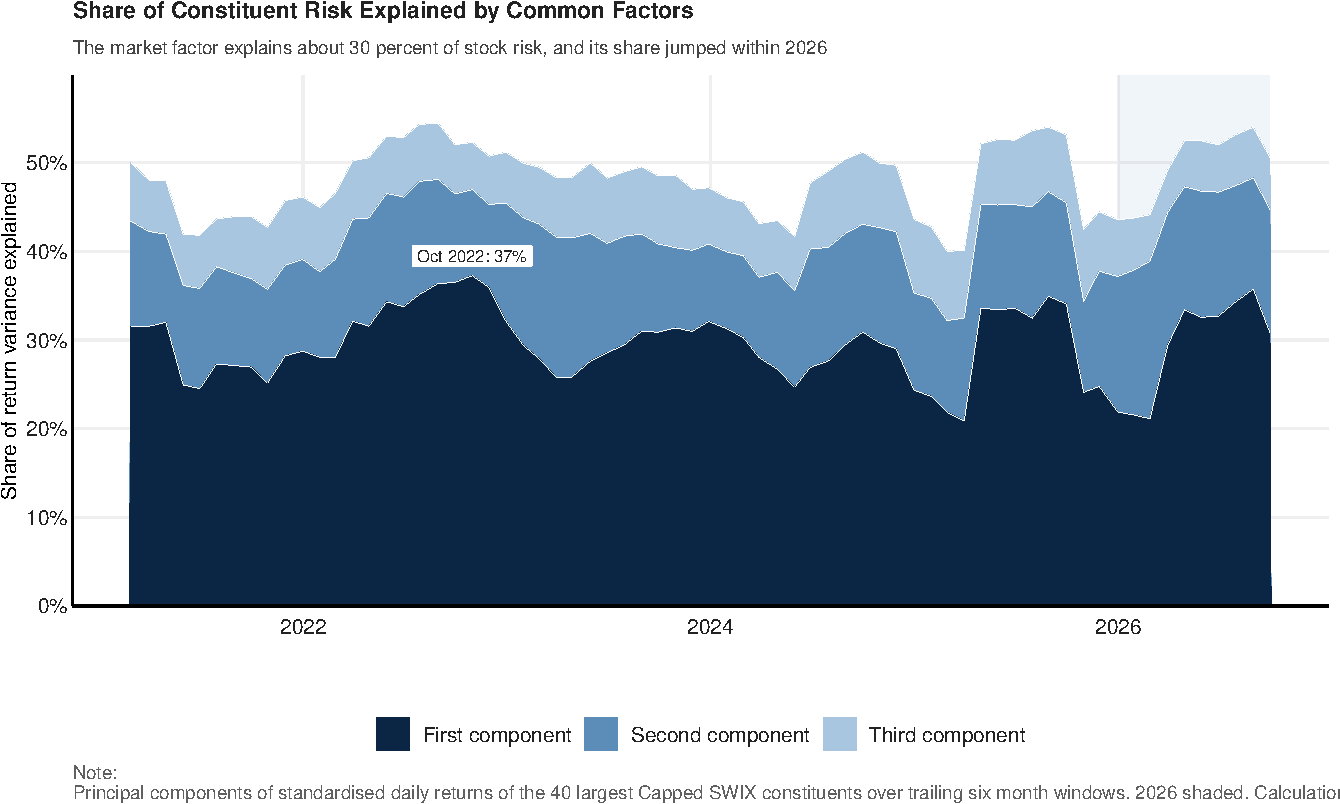
\includegraphics[width=1\linewidth]{Question1_files/figure-latex/q1c_pca-1} 

}

\caption{Share of Constituent Risk Explained by Common Factors}\label{fig:q1c_pca}
\end{figure}

Figure \ref{fig:q1c_pca} shows the share of constituent variance
explained by the first three principal components. The first component
explained 29.5 percent on average before 2026 and 30.2 percent in 2026,
but rose sharply within the year, from 21.1 percent to 35.7 percent, in
line with the correlation result.

\subsection{Opportunity and Active Manager
Outcomes}\label{opportunity-and-active-manager-outcomes}

A wider opportunity set should allow skilled managers to separate from
the rest. The figure relates the trailing 12 month average of weighted
dispersion to the spread of 12 month excess returns across South African
active managers, and colours each month by the share of managers who
beat the Capped SWIX over that year. The points are connected in time
order.

\begin{figure}[H]

{\centering 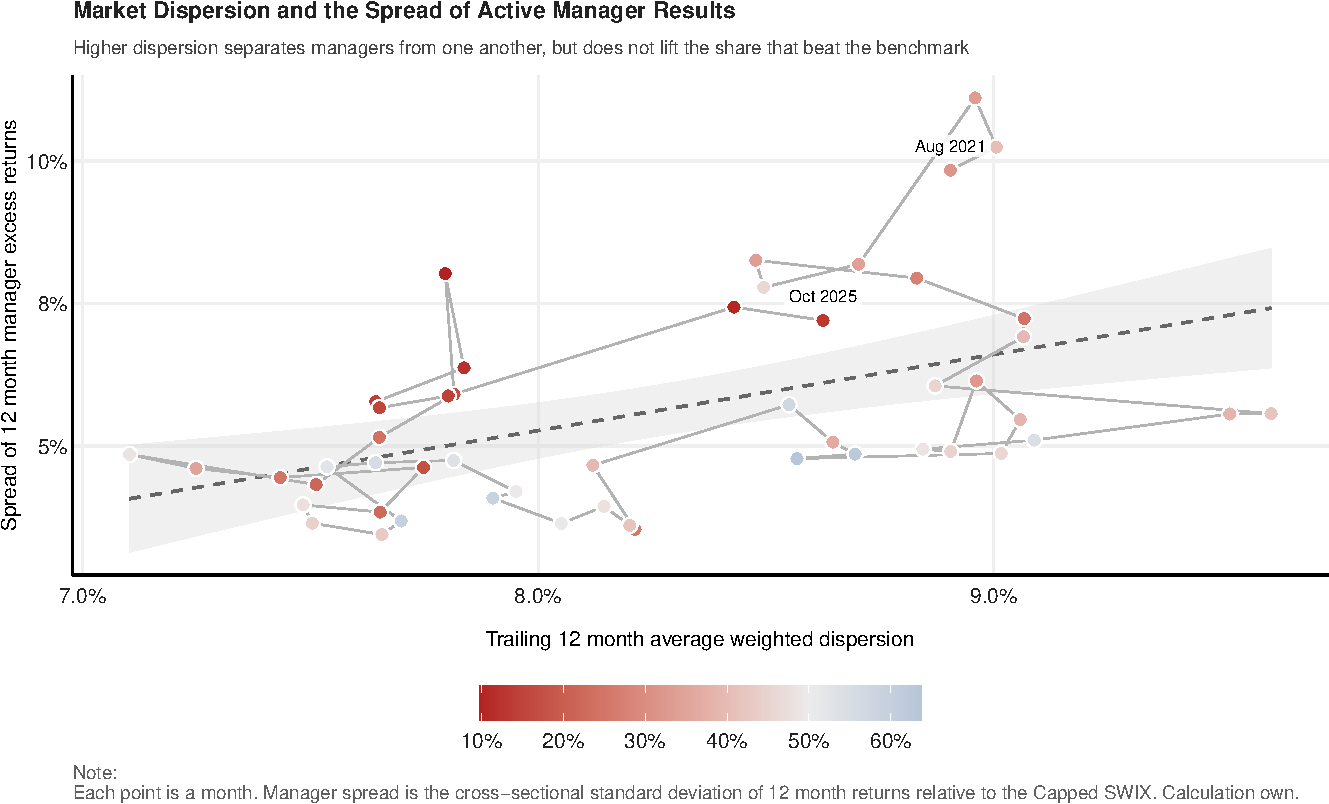
\includegraphics[width=1\linewidth]{Question1_files/figure-latex/q1c_managers-1} 

}

\caption{Market Dispersion and the Spread of Active Manager Results}\label{fig:q1c_managers}
\end{figure}

Over the 51 months for which both series exist, trailing dispersion has
a correlation of 0.48 with the spread of manager excess returns, so
managers' results diverged more when the market offered more dispersion.
The opportunity is real, in the sense that portfolios that differ from
the benchmark produce more different outcomes when stocks diverge. The
correlation with the share of managers beating the benchmark is only
0.14, however, and the colours show that most months are red. In 80
percent of months fewer than half of managers were ahead of the index,
regardless of the level of dispersion. Higher dispersion therefore
raises the stakes of active management without raising the average
manager's success rate, which is what one would expect if skill is
scarce and fees are a constant drag.

\subsection{Manager Outcomes by Dispersion
Regime}\label{manager-outcomes-by-dispersion-regime}

\begin{figure}[H]

{\centering 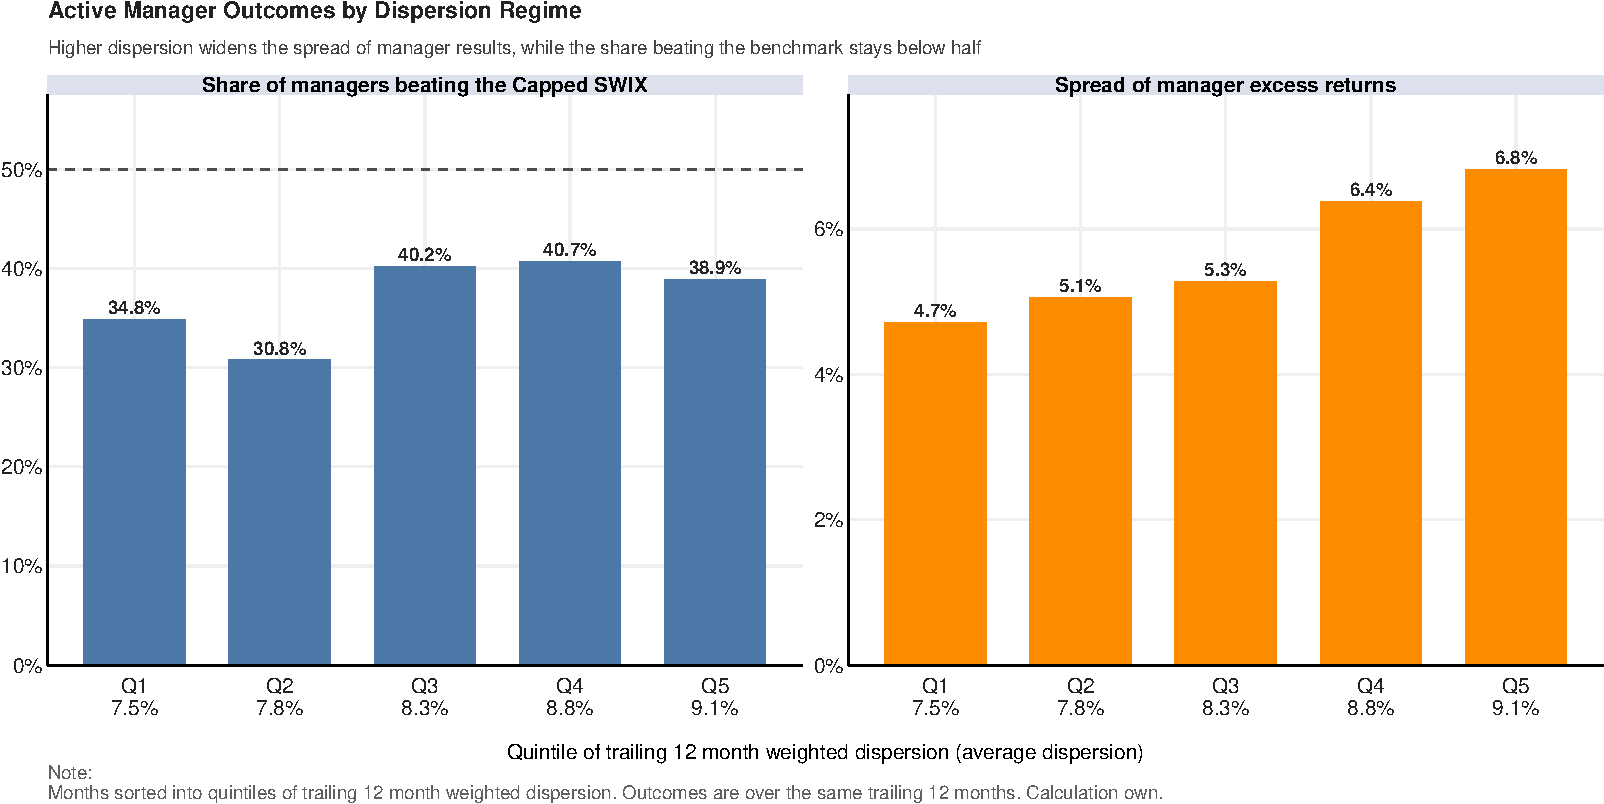
\includegraphics[width=1\linewidth]{Question1_files/figure-latex/q1c_regimes-1} 

}

\caption{Active Manager Outcomes by Dispersion Regime}\label{fig:q1c_regimes}
\end{figure}

Figure \ref{fig:q1c_regimes} groups the months into dispersion
quintiles. The spread of manager results rises from 4.7 percent to 6.8
percent, while the share beating the benchmark stays below half in every
regime. Dispersion raises the stakes of active management without
raising the typical manager's success rate.

\subsection{Alpha Opportunity and the Global Macro
Backdrop}\label{alpha-opportunity-and-the-global-macro-backdrop}

\begin{figure}[H]

{\centering 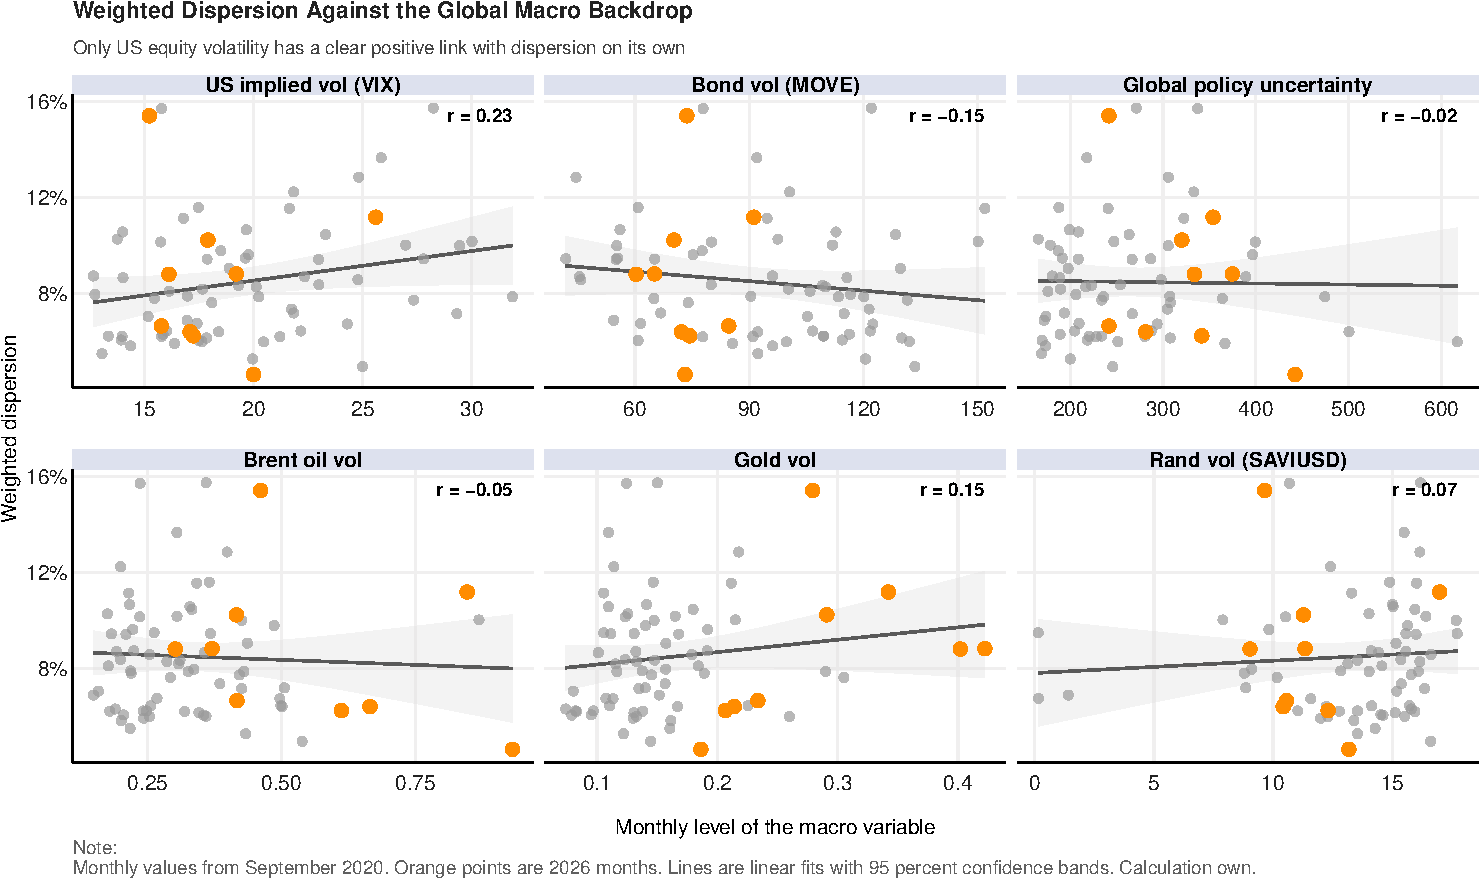
\includegraphics[width=1\linewidth]{Question1_files/figure-latex/q1c_macro_scatter-1} 

}

\caption{Weighted Dispersion Against the Global Macro Backdrop}\label{fig:q1c_macro_scatter}
\end{figure}

Figure \ref{fig:q1c_macro_scatter} relates weighted dispersion to six
macro variables one at a time. Only US equity volatility shows a clear
positive link on its own, and the 2026 months sit across the range of
every variable.

\subsection{Multiple Regression on the Macro
Variables}\label{multiple-regression-on-the-macro-variables}

Because the macro variables are themselves related, a multiple
regression is needed to isolate the effect of each. Both dispersion and
implied correlation are regressed on the six standardised variables, so
that each coefficient is the effect of a one standard deviation move.
Newey-West standard errors are used because the rolling windows overlap
from month to month, which makes the residuals autocorrelated and would
otherwise overstate significance. The largest correlation between any
two regressors is 0.42, so multicollinearity is modest.

\begin{figure}[H]

{\centering 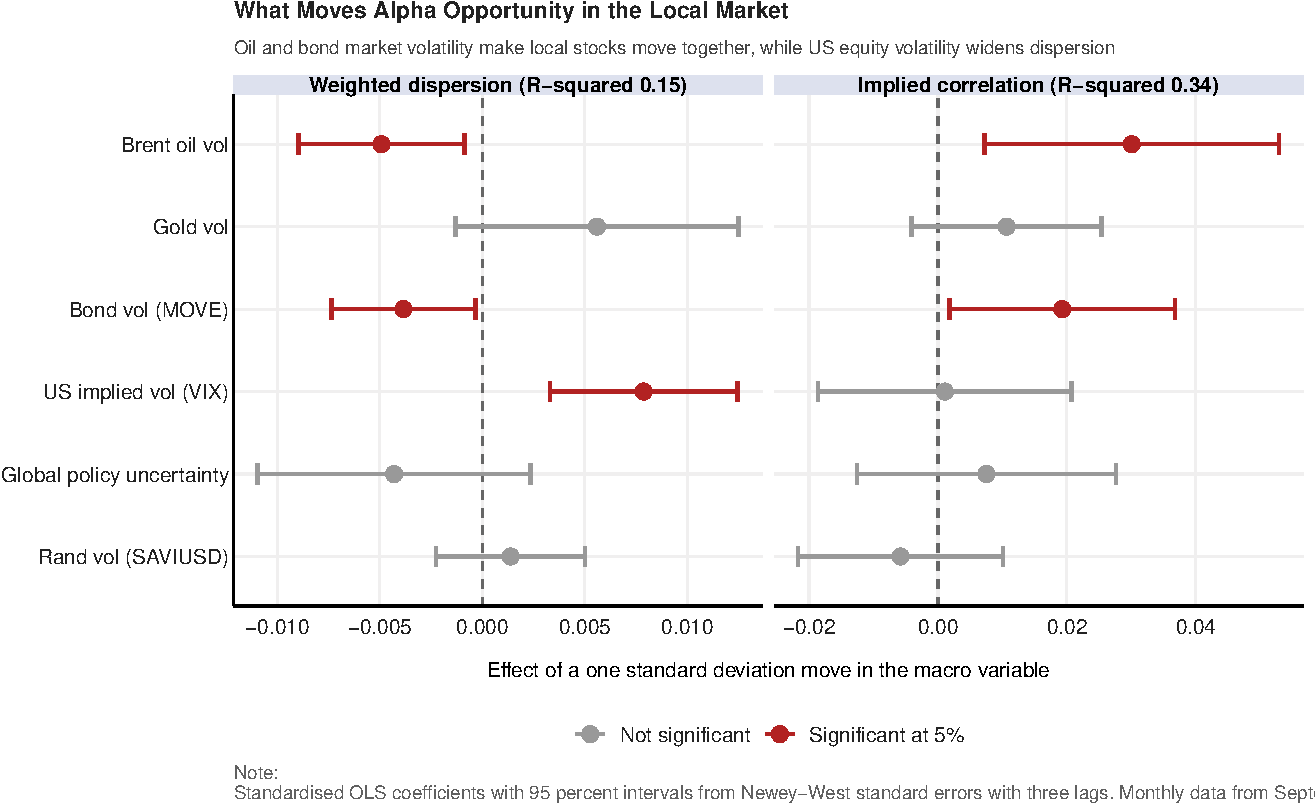
\includegraphics[width=1\linewidth]{Question1_files/figure-latex/q1c_macro_regression-1} 

}

\caption{What Moves Alpha Opportunity in the Local Market}\label{fig:q1c_macro_regression}
\end{figure}

The regressions separate the macro drivers more clearly than the scatter
plots. Implied correlation is the better explained of the two, with an
R-squared of 0.34, and its significant drivers are oil volatility and
bond market volatility. A one standard deviation rise in oil volatility
raises the implied correlation by 0.03, and the same move in the MOVE
index raises it by 0.02. Both are shocks that hit the whole local market
at once, through commodity prices and the global cost of capital, so
they push local stocks to move as a block and shrink the opportunity to
stand out. The same two variables reduce dispersion once the VIX is held
constant, while the VIX itself is the one significant positive driver of
dispersion, adding 0.79 percentage points to dispersion per standard
deviation. The dispersion model explains only 15 percent of the
variation, however, which is consistent with dispersion being dominated
by stock-specific events such as the Naspers buyback and the gold rally.
Global policy uncertainty is insignificant in both models, which matches
the finding in Part A that news-based uncertainty matters only once it
reaches a market price.

\subsection{Summary of Part C}\label{summary-of-part-c}

The alpha opportunity in the local market since 2020 has been episodic,
with no clear trend. Weighted dispersion has hovered around 8 to 9
percent, punctuated by sharp spikes when heavyweight stocks made large
idiosyncratic moves, and the most favourable environment for stock
pickers came in mid 2025, when correlations fell below 0.1 and more than
90 percent of stock risk was diversifiable. In 2026 conditions for stock
picking deteriorated in a less obvious way. Stock volatility rose, but
the largest stocks moved together more closely than at any point in the
sample, so a larger share of the extra risk was common to the market and
could not be avoided by stock selection.

The macro evidence explains why. Oil and bond market volatility, the
channels through which offshore shocks reach the local market, raise
correlations and compress the opportunity set, while broader US equity
volatility tends to widen dispersion. For the team, this links the three
parts of the question. The commodity and rate shocks that drove local
volatility in Part A are the same forces that reduce the room for active
management, and SafeCore's concentration in gold miners in Part B left
it exposed to exactly the kind of common, correlated risk that dominated
2026. A risk ballast built from diversifying holdings would therefore
have helped on both fronts, by lowering volatility and by preserving the
fund's ability to differ from the market when correlations rise.

\FloatBarrier

\section{\texorpdfstring{Conclusion
\label{Conclusion}}{Conclusion }}\label{conclusion}

Local volatility increased in 2026, but as a temporary episode that
followed emerging markets and the oil market, while developed market
volatility stayed below its average. Market-based stress transmits
offshore uncertainty to local shares, while news-based policy
uncertainty on its own does not. SafeCore outperformed its benchmark
through stock selection, yet it did not manage volatility, offered no
protection in stressed months, held no low volatility exposure and
became concentrated in two gold miners. The vendor's volatility score
cannot identify a defensive portfolio, while a score built from realised
volatility can. Finally, the oil and bond market volatility that carries
offshore shocks into the local market also raises correlations among the
largest stocks, which shrinks the room for active management. A low
volatility sleeve built from realised volatility, together with a limit
on any single stock's contribution to risk, would give SafeCore a
ballast against exactly the shocks that dominated 2026.

\bibliography{Tex/ref}





\end{document}
